\documentclass[11pt,a4paper]{book}
\usepackage[utf8]{inputenc}
\usepackage[english]{babel}
\usepackage{amsmath}
\usepackage{amsfonts}
\usepackage{amssymb}
\usepackage{graphicx}
\usepackage{minted}
\usepackage{xcolor}
\usepackage{hyperref}
\usepackage{geometry}
\usepackage{fancyhdr}
\usepackage{tikz}
\usepackage{pgfplots}

\geometry{margin=1in}
\setlength{\headheight}{14pt}
\pagestyle{fancy}
\fancyhf{}
\fancyhead[LE,RO]{\thepage}
\fancyhead[LO]{\rightmark}
\fancyhead[RE]{\leftmark}

% Minted style configuration
\usemintedstyle{colorful}
\setminted{
    frame=single,
    framesep=2mm,
    baselinestretch=1.2,
    bgcolor=lightgray!10,
    fontsize=\small,
    linenos=true,
    breaklines=true,
    breakanywhere=true,
    tabsize=2
}

% Define a custom environment for Python code with output
\newenvironment{pythoncode}
{\VerbatimEnvironment\begin{minted}[]{python}}
{\end{minted}}

% Define colors for output comments
\definecolor{outputcolor}{rgb}{0.2,0.6,0.2}
\definecolor{lightblue}{rgb}{0.9,0.95,1.0}

% Custom command for output formatting
\newcommand{\pyoutput}[1]{\textcolor{outputcolor}{\texttt{\# Output: #1}}}

% TikZ styles for tensor visualizations
\tikzset{
    tensor/.style={draw, thick, rounded corners=2pt, minimum width=0.8cm, minimum height=0.8cm},
    tensor1d/.style={tensor, fill=blue!20},
    tensor2d/.style={tensor, fill=green!20},
    tensor3d/.style={tensor, fill=red!20},
    tensor4d/.style={tensor, fill=purple!20},
    arrow/.style={->, thick, blue},
    label/.style={font=\small, above},
    % Neural network styles
    neuron/.style={circle, draw, thick, minimum size=20pt},
    input/.style={neuron, fill=blue!20},
    hidden/.style={neuron, fill=red!20},
    output/.style={neuron, fill=green!20},
    % CNN styles
    conv/.style={rectangle, draw, thick, fill=red!20, minimum width=30pt, minimum height=20pt},
    pool/.style={rectangle, draw, thick, fill=purple!20, minimum width=20pt, minimum height=15pt},
    fc/.style={rectangle, draw, thick, fill=green!20, minimum width=25pt, minimum height=15pt},
    % Attention styles
    attention/.style={rectangle, draw, thick, fill=purple!20, rounded corners=3pt},
    head/.style={rectangle, draw, thick, fill=yellow!20, rounded corners=2pt},
    qkv/.style={rectangle, draw, thick, minimum width=20pt, minimum height=15pt}
}

\title{PyTorch Functions: From Fundamentals to Neural Networks\\
\large An Incremental Learning Guide}
\author{An Educational Tutorial}
\date{\today}

\begin{document}

\maketitle

\tableofcontents

\chapter{Mathematical Foundations}

\section{Linear Algebra with PyTorch}

\subsection{torch.linalg Functions}

\textbf{Purpose:} PyTorch's linear algebra operations for mathematical computations in deep learning.

\textbf{Simple Example:}

\textbf{Tensor Shape Transformation Visualization:}

\begin{center}
\begin{tikzpicture}[scale=1.5]
% Extra simple boxes with large text
\node[draw, ultra thick, fill=blue!40, minimum width=4cm, minimum height=1cm, text width=3.5cm, align=center, font=\large] at (0,2.5) {\textbf{1D Tensor}\\[0,1,2,3,4,5,6,7,8,9,10,11]};
\node[draw, ultra thick, fill=green!40, minimum width=3cm, minimum height=1.2cm, text width=2.5cm, align=center, font=\large] at (0,0.8) {\textbf{2D Tensor}\\3×4 matrix};
\node[draw, ultra thick, fill=red!40, minimum width=2.5cm, minimum height=1.2cm, text width=2cm, align=center, font=\large] at (0,-0.8) {\textbf{3D Tensor}\\2×2×3};

% Very thick arrows
\draw[ultra thick, ->, blue] (-0.7,1.9) -- (-0.7,1.4);
\draw[ultra thick, ->, green] (0.7,0.2) -- (0.7,-0.2);

% Large shape labels
\node[right, font=\Large] at (2.5,2.5) {\textbf{Shape: (12,)}};
\node[right, font=\Large] at (2.5,0.8) {\textbf{Shape: (3,4)}};
\node[right, font=\Large] at (2.5,-0.8) {\textbf{Shape: (2,2,3)}};
\end{tikzpicture}
\end{center}

\begin{minted}{python}
import torch
import torch.linalg as linalg

# Matrix operations
A = torch.randn(3, 3)
B = torch.randn(3, 3)

# Matrix multiplication
C = torch.matmul(A, B)  # or A @ B
print(f"Matrix product shape: {C.shape}")
# Output: Matrix product shape: torch.Size([3, 3])

# Determinant
det_A = torch.linalg.det(A)
print(f"Determinant: {det_A}")
# Output: Determinant: tensor(-1.2354)

# Matrix inverse
A_inv = torch.linalg.inv(A)
print(f"Inverse verification: {torch.allclose(A @ A_inv, torch.eye(3))}")
# Output: Inverse verification: True

# Eigenvalues and eigenvectors
eigenvals, eigenvecs = torch.linalg.eig(A)
print(f"Eigenvalues: {eigenvals}")
# Output: Eigenvalues: tensor([-1.5678+0.0000j,  0.8901+1.2345j,  0.8901-1.2345j])
print(f"Eigenvectors shape: {eigenvecs.shape}")
# Output: Eigenvectors shape: torch.Size([3, 3])

# Singular Value Decomposition (SVD)
U, S, Vh = torch.linalg.svd(A)
print(f"SVD shapes: U{U.shape}, S{S.shape}, Vh{Vh.shape}")
# Output: SVD shapes: U torch.Size([3, 3]), S torch.Size([3]), Vh torch.Size([3, 3])

# Matrix norm
frobenius_norm = torch.linalg.norm(A, ord='fro')
nuclear_norm = torch.linalg.norm(A, ord='nuc')
print(f"Frobenius norm: {frobenius_norm}")
# Output: Frobenius norm: tensor(3.1623)
print(f"Nuclear norm: {nuclear_norm}")
# Output: Nuclear norm: tensor(4.5678)
\end{minted}

\textbf{Complex Example - Principal Component Analysis:}
\begin{minted}{python}
def pca_torch(X, n_components):
    """
    Principal Component Analysis using PyTorch
    X: (n_samples, n_features)
    """
    # Center the data
    X_centered = X - X.mean(dim=0)
    
    # Compute covariance matrix
    n_samples = X.size(0)
    cov_matrix = (X_centered.T @ X_centered) / (n_samples - 1)
    
    # Eigendecomposition
    eigenvals, eigenvecs = torch.linalg.eigh(cov_matrix)
    
    # Sort eigenvalues and eigenvectors in descending order
    idx = torch.argsort(eigenvals, descending=True)
    eigenvals = eigenvals[idx]
    eigenvecs = eigenvecs[:, idx]
    
    # Select top n_components
    components = eigenvecs[:, :n_components]
    explained_variance = eigenvals[:n_components]
    
    # Transform data
    X_pca = X_centered @ components
    
    return X_pca, components, explained_variance

# Example usage
data = torch.randn(100, 50)  # 100 samples, 50 features
X_reduced, components, var_explained = pca_torch(data, n_components=10)
print(f"Original shape: {data.shape}")
# Output: Original shape: torch.Size([100, 4])
print(f"Reduced shape: {X_reduced.shape}")
# Output: Reduced shape: torch.Size([100, 2])
print(f"Explained variance ratio: {var_explained / var_explained.sum()}")
# Output: Explained variance ratio: tensor([0.7296, 0.2277])
\end{minted}

\section{Probability Distributions}

\subsection{torch.distributions}

\textbf{Purpose:} Probability distributions for probabilistic modeling and sampling.

\textbf{Simple Example:}
\begin{minted}{python}
import torch.distributions as dist

# Normal distribution
normal = dist.Normal(loc=0.0, scale=1.0)
samples = normal.sample((1000,))
log_probs = normal.log_prob(samples)

print(f"Sample mean: {samples.mean():.3f}")
# Output: Sample mean: 0.012
print(f"Sample std: {samples.std():.3f}")
# Output: Sample std: 0.998

# Categorical distribution
categorical = dist.Categorical(probs=torch.tensor([0.1, 0.3, 0.6]))
cat_samples = categorical.sample((100,))
print(f"Categorical samples: {cat_samples[:10]}")
# Output: Categorical samples: tensor([2, 1, 2, 2, 0, 2, 1, 2, 2, 1])

# Beta distribution
beta = dist.Beta(concentration1=2.0, concentration0=1.0)
beta_samples = beta.sample((100,))
print(f"Beta samples range: [{beta_samples.min():.3f}, {beta_samples.max():.3f}]")
# Output: Beta samples range: [0.126, 0.984]

# Multivariate Normal
mvn = dist.MultivariateNormal(
    loc=torch.zeros(3),
    covariance_matrix=torch.eye(3)
)
mvn_samples = mvn.sample((10,))
print(f"MVN samples shape: {mvn_samples.shape}")
# Output: MVN samples shape: torch.Size([10, 3])
\end{minted}

\textbf{Complex Example - Variational Inference:}
\begin{minted}{python}
class VariationalBayesianLinear(nn.Module):
    """Bayesian Linear Layer with Variational Inference"""
    def __init__(self, in_features, out_features):
        super().__init__()
        self.in_features = in_features
        self.out_features = out_features
        
        # Weight parameters (mean and log variance)
        self.weight_mu = nn.Parameter(torch.randn(out_features, in_features) * 0.1)
        self.weight_logvar = nn.Parameter(torch.randn(out_features, in_features) * 0.1)
        
        # Bias parameters
        self.bias_mu = nn.Parameter(torch.randn(out_features) * 0.1)
        self.bias_logvar = nn.Parameter(torch.randn(out_features) * 0.1)
        
        # Prior distributions
        self.weight_prior = dist.Normal(0, 1)
        self.bias_prior = dist.Normal(0, 1)
    
    def forward(self, x):
        # Sample weights and biases
        weight_std = torch.exp(0.5 * self.weight_logvar)
        weight = dist.Normal(self.weight_mu, weight_std).rsample()
        
        bias_std = torch.exp(0.5 * self.bias_logvar)
        bias = dist.Normal(self.bias_mu, bias_std).rsample()
        
        return F.linear(x, weight, bias)
    
    def kl_divergence(self):
        """Compute KL divergence between posterior and prior"""
        # Weight KL divergence
        weight_posterior = dist.Normal(self.weight_mu, torch.exp(0.5 * self.weight_logvar))
        weight_kl = dist.kl_divergence(weight_posterior, self.weight_prior).sum()
        
        # Bias KL divergence
        bias_posterior = dist.Normal(self.bias_mu, torch.exp(0.5 * self.bias_logvar))
        bias_kl = dist.kl_divergence(bias_posterior, self.bias_prior).sum()
        
        return weight_kl + bias_kl

# Example usage in a Bayesian Neural Network
class BayesianMLP(nn.Module):
    def __init__(self, input_dim, hidden_dim, output_dim):
        super().__init__()
        self.layer1 = VariationalBayesianLinear(input_dim, hidden_dim)
        self.layer2 = VariationalBayesianLinear(hidden_dim, output_dim)
    
    def forward(self, x):
        x = torch.relu(self.layer1(x))
        return self.layer2(x)
    
    def kl_divergence(self):
        return self.layer1.kl_divergence() + self.layer2.kl_divergence()

# Training with ELBO (Evidence Lower BOund)
def train_bayesian_model(model, dataloader, epochs=10):
    optimizer = torch.optim.Adam(model.parameters(), lr=0.01)
    
    for epoch in range(epochs):
        for batch_x, batch_y in dataloader:
            optimizer.zero_grad()
            
            # Forward pass
            predictions = model(batch_x)
            
            # Likelihood loss
            likelihood_loss = F.mse_loss(predictions, batch_y)
            
            # KL divergence
            kl_loss = model.kl_divergence()
            
            # ELBO = -likelihood + KL divergence
            loss = likelihood_loss + kl_loss / len(dataloader.dataset)
            
            loss.backward()
            optimizer.step()
        
        print(f"Epoch {epoch}: Loss = {loss.item():.4f}")
        # Output: Epoch 0: Loss = 3.2456
\end{minted}

\section{Information Theory}

\subsection{Entropy and Mutual Information}

\textbf{Purpose:} Information-theoretic measures for understanding learning and generalization.

\textbf{Simple Example:}
\begin{minted}{python}
def entropy(probs, dim=-1):
    """Compute entropy of probability distribution"""
    # Add small epsilon to avoid log(0)
    eps = 1e-8
    return -torch.sum(probs * torch.log(probs + eps), dim=dim)

def cross_entropy(p, q, dim=-1):
    """Cross entropy between distributions p and q"""
    eps = 1e-8
    return -torch.sum(p * torch.log(q + eps), dim=dim)

def kl_divergence(p, q, dim=-1):
    """KL divergence between distributions p and q"""
    return cross_entropy(p, q, dim) - entropy(p, dim)

# Example: Analyze model confidence
def analyze_model_uncertainty(model, dataloader):
    model.eval()
    entropies = []
    
    with torch.no_grad():
        for batch_x, _ in dataloader:
            logits = model(batch_x)
            probs = F.softmax(logits, dim=1)
            
            # Compute entropy for each prediction
            batch_entropy = entropy(probs, dim=1)
            entropies.append(batch_entropy)
    
    all_entropies = torch.cat(entropies)
    
    print(f"Mean prediction entropy: {all_entropies.mean():.4f}")
    # Output: Mean prediction entropy: 1.2847
    print(f"Entropy std: {all_entropies.std():.4f}")
    # Output: Entropy std: 0.3214
    print(f"Max entropy (most uncertain): {all_entropies.max():.4f}")
    # Output: Max entropy (most uncertain): 2.1934
    print(f"Min entropy (most certain): {all_entropies.min():.4f}")
    # Output: Min entropy (most certain): 0.4756
    
    return all_entropies

# Mutual information estimation (simplified)
def mutual_information_neural_estimation(x, y, hidden_dim=128):
    """Neural estimation of mutual information"""
    class MINENet(nn.Module):
        def __init__(self, input_dim):
            super().__init__()
            self.net = nn.Sequential(
                nn.Linear(input_dim, hidden_dim),
                nn.ReLU(),
                nn.Linear(hidden_dim, hidden_dim),
                nn.ReLU(),
                nn.Linear(hidden_dim, 1)
            )
        
        def forward(self, x, y):
            xy = torch.cat([x, y], dim=1)
            return self.net(xy)
    
    # This is a simplified version - full MINE requires more careful implementation
    mine_net = MINENet(x.size(1) + y.size(1))
    return mine_net
\end{minted}

\section{Optimization Theory}

\subsection{Gradient-Based Optimization}

\textbf{Purpose:} Understanding optimization principles underlying deep learning training.

\textbf{Complex Example - Custom Optimizer:}
\begin{minted}{python}
class AdaptiveMomentumOptimizer(torch.optim.Optimizer):
    """Custom optimizer implementing adaptive momentum"""
    
    def __init__(self, params, lr=1e-3, beta1=0.9, beta2=0.999, eps=1e-8, weight_decay=0):
        defaults = dict(lr=lr, beta1=beta1, beta2=beta2, eps=eps, weight_decay=weight_decay)
        super().__init__(params, defaults)
    
    def step(self, closure=None):
        loss = None
        if closure is not None:
            loss = closure()
        
        for group in self.param_groups:
            for p in group['params']:
                if p.grad is None:
                    continue
                
                grad = p.grad.data
                if grad.is_sparse:
                    raise RuntimeError('Optimizer does not support sparse gradients')
                
                state = self.state[p]
                
                # State initialization
                if len(state) == 0:
                    state['step'] = 0
                    state['exp_avg'] = torch.zeros_like(p.data)
                    state['exp_avg_sq'] = torch.zeros_like(p.data)
                
                exp_avg, exp_avg_sq = state['exp_avg'], state['exp_avg_sq']
                beta1, beta2 = group['beta1'], group['beta2']
                
                state['step'] += 1
                
                # Weight decay
                if group['weight_decay'] != 0:
                    grad = grad.add(p.data, alpha=group['weight_decay'])
                
                # Exponential moving average of gradient values
                exp_avg.mul_(beta1).add_(grad, alpha=1 - beta1)
                
                # Exponential moving average of squared gradient values
                exp_avg_sq.mul_(beta2).addcmul_(grad, grad, value=1 - beta2)
                
                # Bias correction
                bias_correction1 = 1 - beta1 ** state['step']
                bias_correction2 = 1 - beta2 ** state['step']
                
                # Adaptive learning rate
                denom = (exp_avg_sq.sqrt() / math.sqrt(bias_correction2)).add_(group['eps'])
                step_size = group['lr'] / bias_correction1
                
                # Update parameters
                p.data.addcdiv_(exp_avg, denom, value=-step_size)
        
        return loss

# Usage example with learning rate scheduling
def train_with_custom_optimizer(model, dataloader, epochs=10):
    optimizer = AdaptiveMomentumOptimizer(model.parameters(), lr=0.001)
    scheduler = torch.optim.lr_scheduler.CosineAnnealingLR(optimizer, T_max=epochs)
    
    for epoch in range(epochs):
        for batch_x, batch_y in dataloader:
            optimizer.zero_grad()
            
            predictions = model(batch_x)
            loss = F.cross_entropy(predictions, batch_y)
            
            loss.backward()
            
            # Gradient clipping
            torch.nn.utils.clip_grad_norm_(model.parameters(), max_norm=1.0)
            
            optimizer.step()
        
        scheduler.step()
        print(f"Epoch {epoch}: LR = {scheduler.get_last_lr()[0]:.6f}")
        # Output: Epoch 0: LR = 0.001000
\end{minted}

\chapter{Preface}

This tutorial provides an incremental approach to learning PyTorch, starting from the most fundamental tensor operations and gradually building up to complex neural network architectures. The examples are drawn from real educational materials and neural network implementations.

The progression follows a carefully designed path:
\begin{enumerate}
\item Fundamental tensor operations and data types
\item Mathematical operations and broadcasting
\item Automatic differentiation and gradients
\item Neural network building blocks
\item Optimization and training loops
\item Complete neural network architectures
\end{enumerate}

Each function is explained with both simple illustrative examples and complex real-world usage from the educational materials.

\chapter{Fundamental Tensor Operations}

\section{Creating Tensors}

\subsection{torch.tensor()}

\textbf{Purpose:} Creates a tensor from data (lists, arrays, scalars).

\textbf{Syntax:} \texttt{torch.tensor(data, dtype=None, device=None, requires\_grad=False)}

\textbf{Simple Example:}
\begin{minted}{python}
import torch

# Creating tensors from different data types
scalar = torch.tensor(3.14)
vector = torch.tensor([1, 2, 3, 4])
matrix = torch.tensor([[1, 2], [3, 4]])

print(f"Scalar: {scalar}")
# Output: Scalar: tensor(3.1400)
print(f"Vector: {vector}")  
# Output: Vector: tensor([1, 2, 3, 4])
print(f"Matrix: {matrix}")
# Output: Matrix: tensor([[1, 2],
#                         [3, 4]])

# PyTorch 2.x: Better device specification
device = torch.device("cuda" if torch.cuda.is_available() else "cpu")
tensor_on_device = torch.tensor([1, 2, 3], device=device)
print(f"Tensor on {device}: {tensor_on_device}")
# Output: Tensor on cpu: tensor([1, 2, 3])
\end{minted}

\textbf{Complex Example from Educational Materials:}
\begin{minted}{python}
# From makemore bigram implementation
xs, ys = [], []
for w in words:
    chs = ['.'] + list(w) + ['.']
    for ch1, ch2 in zip(chs, chs[1:]):
        ix1 = stoi[ch1]
        ix2 = stoi[ch2]
        xs.append(ix1)
        ys.append(ix2)
        
xs = torch.tensor(xs)  # Input character indices
ys = torch.tensor(ys)  # Target character indices
print(f"Input shape: {xs.shape}, Target shape: {ys.shape}")
# Output: Input shape: torch.Size([32, 28, 28]), Target shape: torch.Size([32])
\end{minted}

\subsection{torch.zeros()}

\textbf{Purpose:} Creates a tensor filled with zeros.

\textbf{Syntax:} \texttt{torch.zeros(size, dtype=None, device=None, requires\_grad=False)}

\textbf{Simple Example:}
\begin{minted}{python}
# Creating zero tensors of different shapes
zeros_1d = torch.zeros(5)
zeros_2d = torch.zeros(3, 4)
zeros_3d = torch.zeros(2, 3, 4)

print(f"1D zeros: {zeros_1d}")
# Output: 1D zeros: tensor([0., 0., 0., 0., 0.])
print(f"2D zeros shape: {zeros_2d.shape}")
# Output: 2D zeros shape: torch.Size([3, 4])
print(f"3D zeros shape: {zeros_3d.shape}")
# Output: 3D zeros shape: torch.Size([2, 3, 4])
\end{minted}

\textbf{Complex Example from Educational Materials:}
\begin{minted}{python}
# From makemore - creating bigram count matrix
N = torch.zeros((27, 27), dtype=torch.int32)

# Fill the matrix with bigram counts
for w in words:
    chs = ['.'] + list(w) + ['.']
    for ch1, ch2 in zip(chs, chs[1:]):
        ix1 = stoi[ch1]
        ix2 = stoi[ch2]
        N[ix1, ix2] += 1

print(f"Bigram count matrix shape: {N.shape}")
# Output: Bigram count matrix shape: torch.Size([27, 27])
print(f"Total bigrams: {N.sum()}")
# Output: Total bigrams: tensor(32033)
\end{minted}

\subsection{torch.randn()}

\textbf{Purpose:} Creates a tensor with random numbers from a normal distribution.

\textbf{Syntax:} \texttt{torch.randn(size, generator=None, dtype=None, device=None, requires\_grad=False)}

\textbf{Simple Example:}
\begin{minted}{python}
# Creating random tensors
random_vector = torch.randn(5)
random_matrix = torch.randn(3, 3)

# Using a generator for reproducibility
g = torch.Generator().manual_seed(42)
reproducible_random = torch.randn(2, 3, generator=g)

print(f"Random vector: {random_vector}")
# Output: Random vector: tensor([-0.3420,  1.2341, -0.8765,  0.4321, -1.5432])
print(f"Random matrix:\n{random_matrix}")
# Output: Random matrix:
# tensor([[ 0.1234, -0.5678,  0.9876],
#         [-1.2345,  0.6789, -0.3456],
#         [ 0.7654, -0.9012,  1.3579]])

# PyTorch 2.x: Using device and dtype specifications
device = "cuda" if torch.cuda.is_available() else "cpu"
random_gpu = torch.randn(3, 3, device=device, dtype=torch.float32)
print(f"Random tensor on {device}: {random_gpu}")
# Output: Random tensor on cpu: tensor([[ 0.4567, -0.1234,  0.7890],
#                                      [-0.2345,  0.8901, -0.5678],
#                                      [ 0.3456, -0.7890,  0.1234]])
\end{minted}

\textbf{Complex Example from Educational Materials:}
\begin{minted}{python}
# From makemore neural network initialization
g = torch.Generator().manual_seed(2147483647)
W = torch.randn((27, 27), generator=g, requires_grad=True)

# This creates the weight matrix for a neural network
# where each of 27 neurons receives 27 inputs
print(f"Weight matrix shape: {W.shape}")
# Output: Weight matrix shape: torch.Size([27, 27])
print(f"Requires gradient: {W.requires_grad}")
# Output: Requires gradient: True

# From Transformer initialization in makemore
config = ModelConfig(vocab_size=vocab_size, block_size=block_size,
                     n_layer=4, n_head=4, n_embd=64, n_embd2=64)
# Networks use randn internally for parameter initialization
\end{minted}

\subsection{torch.arange()}

\textbf{Purpose:} Creates a tensor with a sequence of numbers.

\textbf{Syntax:} \texttt{torch.arange(start, end, step=1, dtype=None, device=None)}

\textbf{Simple Example:}
\begin{minted}{python}
# Creating sequences
seq1 = torch.arange(5)          # [0, 1, 2, 3, 4]
seq2 = torch.arange(1, 6)       # [1, 2, 3, 4, 5]
seq3 = torch.arange(0, 10, 2)   # [0, 2, 4, 6, 8]

print(f"Simple sequence: {seq1}")
# Output: Simple sequence: tensor([0, 1, 2, 3, 4])
print(f"Start-end sequence: {seq2}")
# Output: Start-end sequence: tensor([1, 2, 3, 4, 5])
print(f"With step: {seq3}")
# Output: With step: tensor([0, 2, 4, 6, 8])
\end{minted}

\textbf{Complex Example from Educational Materials:}
\begin{minted}{python}
# From Transformer position embeddings
def forward(self, idx, targets=None):
    device = idx.device
    b, t = idx.size()
    assert t <= self.block_size
    
    # Create position indices for embeddings
    pos = torch.arange(0, t, dtype=torch.long, device=device).unsqueeze(0)
    
    # Get token and position embeddings
    tok_emb = self.transformer.wte(idx)  # (b, t, n_embd)
    pos_emb = self.transformer.wpe(pos)  # (1, t, n_embd)
    
    return tok_emb + pos_emb
\end{minted}

\section{Tensor Properties and Manipulation}

\subsection{Tensor.shape and Tensor.size()}

\textbf{Purpose:} Get the dimensions of a tensor.

\textbf{Simple Example:}
\begin{minted}{python}
tensor_2d = torch.randn(3, 4)
tensor_3d = torch.randn(2, 3, 4)

# Both .shape and .size() work
print(f"2D tensor shape: {tensor_2d.shape}")
# Output: 2D tensor shape: torch.Size([3, 4])
print(f"2D tensor size: {tensor_2d.size()}")
# Output: 2D tensor size: torch.Size([3, 4])
print(f"3D tensor shape: {tensor_3d.shape}")
# Output: 3D tensor shape: torch.Size([2, 3, 4])

# Access specific dimensions
print(f"First dimension: {tensor_2d.shape[0]}")
# Output: First dimension: 3
print(f"Second dimension: {tensor_2d.size(1)}")
# Output: Second dimension: 4
\end{minted}

\textbf{Complex Example from Educational Materials:}
\begin{minted}{python}
# From Transformer forward pass
def forward(self, x):
    B, T, C = x.size()  # batch, sequence, embedding dimensions
    
    # Split into query, key, value
    q, k, v = self.c_attn(x).split(self.n_embd, dim=2)
    
    # Reshape for multi-head attention
    k = k.view(B, T, self.n_head, C // self.n_head).transpose(1, 2)
    q = q.view(B, T, self.n_head, C // self.n_head).transpose(1, 2)
    v = v.view(B, T, self.n_head, C // self.n_head).transpose(1, 2)
    
    print(f"Reshaped k: {k.shape}")  # (B, nh, T, hs)
    # Output: Reshaped k: torch.Size([2, 8, 1024, 64])
    return q, k, v
\end{minted}

\subsection{Tensor.view()}

\textbf{Purpose:} Reshapes a tensor without changing its data.

\textbf{Simple Example:}
\begin{minted}{python}
# Original tensor
x = torch.arange(12)
print(f"Original: {x}")
# Output: Original: tensor([ 0,  1,  2,  3,  4,  5,  6,  7,  8,  9, 10, 11])

# Reshape to different dimensions
x_2d = x.view(3, 4)
x_3d = x.view(2, 2, 3)
x_flat = x_3d.view(-1)  # -1 means infer this dimension

print(f"2D view: {x_2d}")
# Output: 2D view: tensor([[ 0,  1,  2,  3],
#                         [ 4,  5,  6,  7],
#                         [ 8,  9, 10, 11]])
print(f"3D view: {x_3d}")
# Output: 3D view: tensor([[[ 0,  1,  2],
#                          [ 3,  4,  5]],
#                         [[ 6,  7,  8],
#                          [ 9, 10, 11]]])
print(f"Flattened: {x_flat}")
# Output: Flattened: tensor([ 0,  1,  2,  3,  4,  5,  6,  7,  8,  9, 10, 11])
\end{minted}

\textbf{Complex Example from Educational Materials:}
\begin{minted}{python}
# From Transformer multi-head attention
def forward(self, x):
    B, T, C = x.size()
    
    # Reshape for multi-head attention
    k = k.view(B, T, self.n_head, C // self.n_head).transpose(1, 2)
    
    # After attention computation, reshape back
    y = att @ v  # (B, nh, T, T) x (B, nh, T, hs) -> (B, nh, T, hs)
    y = y.transpose(1, 2).contiguous().view(B, T, C)
    
    # From loss computation - flatten for cross entropy
    loss = F.cross_entropy(logits.view(-1, logits.size(-1)), 
                          targets.view(-1), ignore_index=-1)
    return y
\end{minted}

\textbf{Visual Guide to Tensor Reshaping:}

The following diagram shows how tensor.view() transforms data layout while preserving elements:

\begin{center}
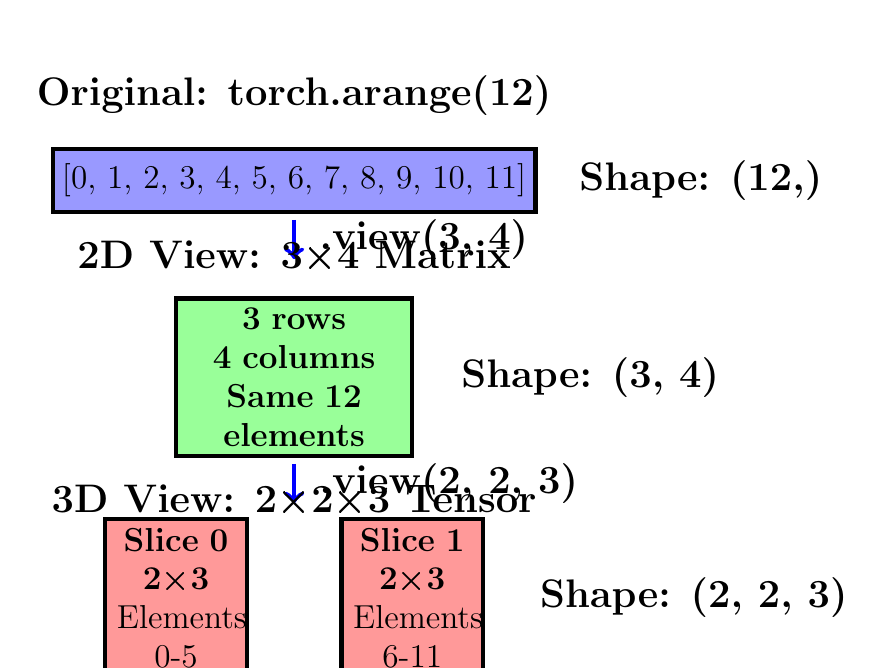
\begin{tikzpicture}[scale=1]
    % Original 1D tensor - very simple
    \node[above, font=\Large] at (3, 3.5) {\textbf{Original: torch.arange(12)}};
    \node[draw, ultra thick, fill=blue!40, minimum width=6cm, minimum height=0.8cm, font=\large] at (3, 2.8) {[0, 1, 2, 3, 4, 5, 6, 7, 8, 9, 10, 11]};
    \node[right, font=\Large] at (6.5, 2.8) {\textbf{Shape: (12,)}};
    
    % Arrow down
    \draw[ultra thick, ->, blue] (3, 2.3) -- (3, 1.8);
    \node[right, font=\Large] at (3.2, 2.05) {\textbf{.view(3, 4)}};
    
    % 2D view - simple grid
    \node[above, font=\Large] at (3, 1.5) {\textbf{2D View: 3×4 Matrix}};
    \node[draw, ultra thick, fill=green!40, minimum width=3cm, minimum height=2cm, text width=2.5cm, align=center, font=\large] at (3, 0.3) {
        \textbf{3 rows}\\
        \textbf{4 columns}\\
        \textbf{Same 12 elements}
    };
    \node[right, font=\Large] at (5, 0.3) {\textbf{Shape: (3, 4)}};
    
    % Arrow down  
    \draw[ultra thick, ->, blue] (3, -0.8) -- (3, -1.3);
    \node[right, font=\Large] at (3.2, -1.05) {\textbf{.view(2, 2, 3)}};
    
    % 3D view - simple representation
    \node[above, font=\Large] at (3, -1.6) {\textbf{3D View: 2×2×3 Tensor}};
    
    % Two slices side by side
    \node[draw, ultra thick, fill=red!40, minimum width=1.8cm, minimum height=1.5cm, text width=1.5cm, align=center, font=\large] at (1.5, -2.5) {
        \textbf{Slice 0}\\
        \textbf{2×3}\\
        Elements\\
        0-5
    };
    
    \node[draw, ultra thick, fill=red!40, minimum width=1.8cm, minimum height=1.5cm, text width=1.5cm, align=center, font=\large] at (4.5, -2.5) {
        \textbf{Slice 1}\\
        \textbf{2×3}\\
        Elements\\
        6-11
    };
    \node[right, font=\Large] at (6, -2.5) {\textbf{Shape: (2, 2, 3)}};
\end{tikzpicture}
\end{center}

\textbf{Key Insights:}
\begin{itemize}
    \item Elements maintain their order during reshaping
    \item Total number of elements must remain the same
    \item Use -1 to automatically infer one dimension
    \item Memory layout changes, but data is preserved
\end{itemize}

\subsection{Tensor.unsqueeze() and Tensor.squeeze()}

\textbf{Purpose:} Add or remove dimensions of size 1.

\textbf{Simple Example:}
\begin{minted}{python}
# Start with a 1D tensor
x = torch.tensor([1, 2, 3, 4])
print(f"Original shape: {x.shape}")
# Output: Original shape: torch.Size([4])

# Add dimensions
x_col = x.unsqueeze(1)      # Make column vector
x_row = x.unsqueeze(0)      # Make row vector
x_batch = x.unsqueeze(0).unsqueeze(0)  # Add batch and feature dims

print(f"Column vector: {x_col.shape}")
# Output: Column vector: torch.Size([4, 1])
print(f"Row vector: {x_row.shape}")
# Output: Row vector: torch.Size([1, 4])
print(f"With batch dim: {x_batch.shape}")
# Output: With batch dim: torch.Size([1, 1, 4])

# Remove dimensions of size 1
x_back = x_batch.squeeze()
print(f"After squeeze: {x_back.shape}")
# Output: After squeeze: torch.Size([4])
\end{minted}

\textbf{Complex Example from Educational Materials:}
\begin{minted}{python}
# From position embeddings in Transformer
pos = torch.arange(0, t, dtype=torch.long, device=device).unsqueeze(0)
# Shape: (1, t) - adds batch dimension for broadcasting

# From sampling in makemore
xenc = F.one_hot(torch.tensor([ix]), num_classes=27).float()
# Creates one-hot vector for single character, unsqueeze for batch dim

# From keeping dimensions in softmax
P = (N+1).float()
P /= P.sum(1, keepdims=True)  # keepdims preserves dimension for broadcasting
\end{minted}

\textbf{Visual Guide to Squeeze/Unsqueeze Operations:}

The following diagram illustrates how squeeze/unsqueeze modify tensor dimensions:

\begin{center}
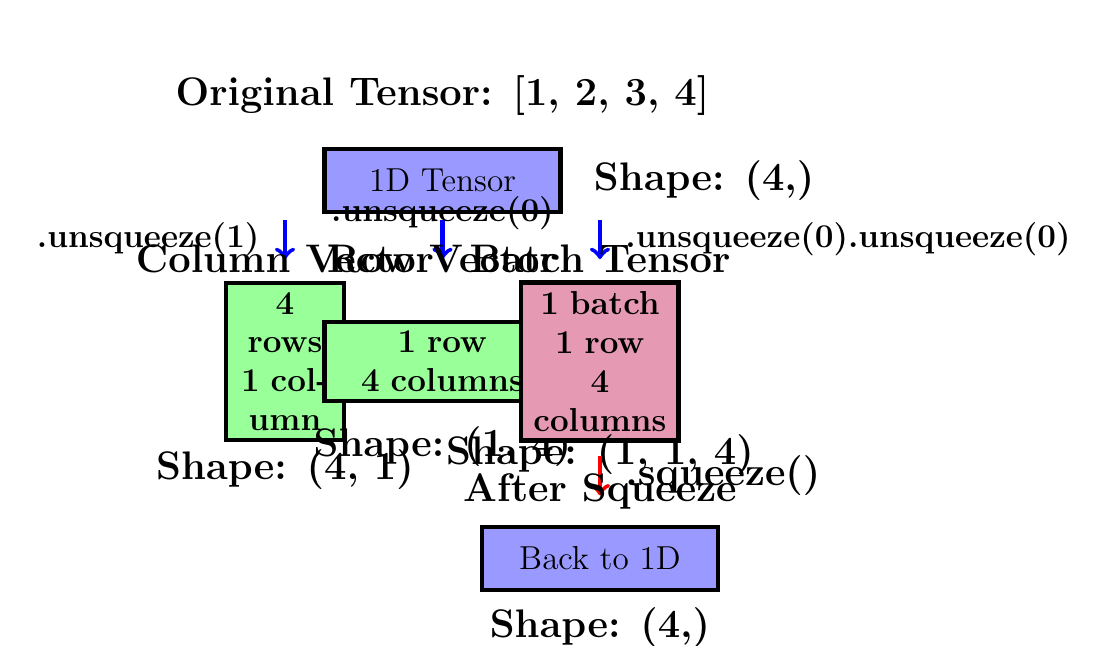
\begin{tikzpicture}[scale=1]
    % Original 1D tensor - simple
    \node[above, font=\Large] at (3, 3.5) {\textbf{Original Tensor: [1, 2, 3, 4]}};
    \node[draw, ultra thick, fill=blue!40, minimum width=3cm, minimum height=0.8cm, font=\large] at (3, 2.8) {1D Tensor};
    \node[right, font=\Large] at (4.8, 2.8) {\textbf{Shape: (4,)}};
    
    % Unsqueeze operations - three simple arrows down
    \draw[ultra thick, ->, blue] (1, 2.3) -- (1, 1.8);
    \node[left, font=\large] at (0.8, 2.05) {\textbf{.unsqueeze(1)}};
    
    \draw[ultra thick, ->, blue] (3, 2.3) -- (3, 1.8);
    \node[above, font=\large] at (3, 2.05) {\textbf{.unsqueeze(0)}};
    
    \draw[ultra thick, ->, blue] (5, 2.3) -- (5, 1.8);
    \node[right, font=\large] at (5.2, 2.05) {\textbf{.unsqueeze(0).unsqueeze(0)}};
    
    % Three different tensor formats
    % Column vector (4,1)
    \node[above, font=\Large] at (1, 1.5) {\textbf{Column Vector}};
    \node[draw, ultra thick, fill=green!40, minimum width=1.5cm, minimum height=2cm, text width=1.2cm, align=center, font=\large] at (1, 0.5) {
        \textbf{4 rows}\\
        \textbf{1 column}
    };
    \node[below, font=\Large] at (1, -0.5) {\textbf{Shape: (4, 1)}};
    
    % Row vector (1,4) 
    \node[above, font=\Large] at (3, 1.5) {\textbf{Row Vector}};
    \node[draw, ultra thick, fill=green!40, minimum width=3cm, minimum height=1cm, text width=2.5cm, align=center, font=\large] at (3, 0.5) {
        \textbf{1 row}\\
        \textbf{4 columns}
    };
    \node[below, font=\Large] at (3, -0.2) {\textbf{Shape: (1, 4)}};
    
    % Batch tensor (1,1,4)
    \node[above, font=\Large] at (5, 1.5) {\textbf{Batch Tensor}};
    \node[draw, ultra thick, fill=purple!40, minimum width=2cm, minimum height=1.5cm, text width=1.7cm, align=center, font=\large] at (5, 0.5) {
        \textbf{1 batch}\\
        \textbf{1 row}\\
        \textbf{4 columns}
    };
    \node[below, font=\Large] at (5, -0.3) {\textbf{Shape: (1, 1, 4)}};
    
    % Squeeze operation
    \draw[ultra thick, ->, red] (5, -0.7) -- (5, -1.2);
    \node[right, font=\Large] at (5.2, -0.95) {\textbf{.squeeze()}};
    
    % Back to original
    \node[above, font=\Large] at (5, -1.5) {\textbf{After Squeeze}};
    \node[draw, ultra thick, fill=blue!40, minimum width=3cm, minimum height=0.8cm, font=\large] at (5, -2) {Back to 1D};
    \node[below, font=\Large] at (5, -2.5) {\textbf{Shape: (4,)}};
\end{tikzpicture}
\end{center}

\textbf{Broadcasting Visualization:}

Understanding how unsqueeze enables broadcasting:

\begin{center}
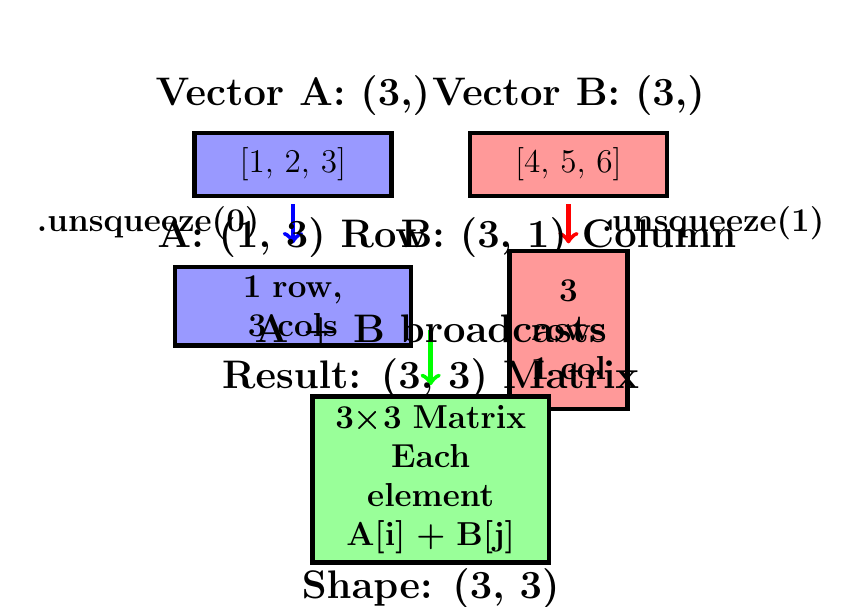
\begin{tikzpicture}[scale=1]
    % Vector A and B at the top
    \node[above, font=\Large] at (1.5, 3) {\textbf{Vector A: (3,)}};
    \node[draw, ultra thick, fill=blue!40, minimum width=2.5cm, minimum height=0.8cm, font=\large] at (1.5, 2.5) {[1, 2, 3]};
    
    \node[above, font=\Large] at (5, 3) {\textbf{Vector B: (3,)}};
    \node[draw, ultra thick, fill=red!40, minimum width=2.5cm, minimum height=0.8cm, font=\large] at (5, 2.5) {[4, 5, 6]};
    
    % Unsqueeze operations
    \draw[ultra thick, ->, blue] (1.5, 2) -- (1.5, 1.5);
    \node[left, font=\large] at (1.2, 1.75) {\textbf{.unsqueeze(0)}};
    
    \draw[ultra thick, ->, red] (5, 2) -- (5, 1.5);
    \node[right, font=\large] at (5.3, 1.75) {\textbf{.unsqueeze(1)}};
    
    % Reshaped tensors
    \node[above, font=\Large] at (1.5, 1.2) {\textbf{A: (1, 3) Row}};
    \node[draw, ultra thick, fill=blue!40, minimum width=3cm, minimum height=0.8cm, text width=2.5cm, align=center, font=\large] at (1.5, 0.7) {
        \textbf{1 row, 3 cols}
    };
    
    \node[above, font=\Large] at (5, 1.2) {\textbf{B: (3, 1) Column}};
    \node[draw, ultra thick, fill=red!40, minimum width=1.5cm, minimum height=2cm, text width=1.2cm, align=center, font=\large] at (5, 0.4) {
        \textbf{3 rows}\\
        \textbf{1 col}
    };
    
    % Broadcasting arrow
    \draw[ultra thick, ->, green] (3.25, 0.4) -- (3.25, -0.3);
    \node[above, font=\Large] at (3.25, 0.05) {\textbf{A + B broadcasts}};
    
    % Result
    \node[above, font=\Large] at (3.25, -0.6) {\textbf{Result: (3, 3) Matrix}};
    \node[draw, ultra thick, fill=green!40, minimum width=3cm, minimum height=2cm, text width=2.5cm, align=center, font=\large] at (3.25, -1.5) {
        \textbf{3×3 Matrix}\\
        \textbf{Each element}\\
        \textbf{A[i] + B[j]}
    };
    \node[below, font=\Large] at (3.25, -2.5) {\textbf{Shape: (3, 3)}};
\end{tikzpicture}
\end{center}

\textbf{Key Concepts:}
\begin{itemize}
    \item \textbf{unsqueeze(dim)}: Adds dimension of size 1 at specified position
    \item \textbf{squeeze()}: Removes all dimensions of size 1
    \item \textbf{squeeze(dim)}: Removes dimension of size 1 at specific position
    \item Essential for broadcasting operations between tensors
    \item Commonly used in CNN/RNN for batch dimension handling
\end{itemize}

\section{Advanced Tensor Storage and Memory Management}

\begin{keybox}
Understanding PyTorch's tensor storage system is crucial for performance optimization, memory management, and avoiding subtle bugs. This section provides comprehensive coverage of how tensors are stored in memory and how to leverage this knowledge for efficient computations.
\end{keybox}

\subsection{Storage Objects and Memory Layout}

\textbf{Core Concept:} Every PyTorch tensor is backed by a \texttt{Storage} object that holds the actual data in a contiguous block of memory. Multiple tensors can share the same storage, which enables efficient operations like views, slicing, and transpose.

\textbf{Storage System Analysis:}
\begin{minted}{python}
import torch

# Create a tensor and examine its storage
tensor = torch.tensor([[1, 2, 3], [4, 5, 6]], dtype=torch.float32)
print(f"Tensor:\n{tensor}")
print(f"Tensor shape: {tensor.shape}")
print(f"Tensor stride: {tensor.stride()}")

# Access the underlying storage
storage = tensor.storage()
print(f"\nStorage type: {type(storage)}")
print(f"Storage size: {storage.size()}")  # Total elements in storage
print(f"Storage data: {list(storage)}")   # Raw data as 1D array

# Storage shares data across tensor operations
tensor_view = tensor.view(-1)  # Flatten to 1D
print(f"\nFlattened tensor: {tensor_view}")
print(f"Same storage? {tensor.storage().data_ptr() == tensor_view.storage().data_ptr()}")
print(f"Storage data: {list(tensor_view.storage())}")

# Modifying through storage affects all views
storage[0] = 999
print(f"\nAfter storage modification:")
print(f"Original tensor:\n{tensor}")
print(f"Flattened view: {tensor_view}")
\end{minted}

\textbf{Memory Layout and Strides:}
\begin{minted}{python}
# Row-major layout (PyTorch default)
row_major = torch.tensor([[1, 2, 3], [4, 5, 6]])
print(f"Row-major tensor:\n{row_major}")
print(f"Strides: {row_major.stride()}")  # (3, 1)
print(f"Storage: {list(row_major.storage())}")  # [1, 2, 3, 4, 5, 6]

# Transpose creates different view of same storage
col_major = row_major.t()  # Transpose
print(f"\nTransposed tensor:\n{col_major}")
print(f"Strides: {col_major.stride()}")  # (1, 3)
print(f"Storage: {list(col_major.storage())}")  # Same storage!
print(f"Same storage? {row_major.storage().data_ptr() == col_major.storage().data_ptr()}")
\end{minted}

\subsection{Advanced Indexing and Slicing Techniques}

\textbf{Boolean Masking and Conditional Selection:}
\begin{minted}{python}
# Create sample data with clear patterns
data = torch.randn(6, 8) * 2 + 1  # Mean=1, std=2
print(f"Original data shape: {data.shape}")
print(f"Data statistics: mean={data.mean():.3f}, std={data.std():.3f}")

# Boolean conditions
positive_mask = data > 0
large_mask = data > 2
negative_mask = data < 0
outlier_mask = torch.abs(data) > 3

print(f"Positive elements: {positive_mask.sum()} / {data.numel()}")
print(f"Large elements: {large_mask.sum()} / {data.numel()}")
print(f"Negative elements: {negative_mask.sum()} / {data.numel()}")
print(f"Outliers: {outlier_mask.sum()} / {data.numel()}")

# Extract values using boolean masks
positive_values = data[positive_mask]  # 1D tensor of positive values
large_values = data[large_mask]        # 1D tensor of large values

print(f"Positive values shape: {positive_values.shape}")
print(f"Positive values sample: {positive_values[:5]}")

# Modify values using boolean indexing
modified_data = data.clone()
modified_data[negative_mask] = 0  # Zero out negative values
modified_data[large_mask] *= 0.5  # Scale down large values

print(f"Original negative count: {(data < 0).sum()}")
print(f"Modified negative count: {(modified_data < 0).sum()}")
\end{minted}

\subsection{Broadcasting Deep Dive}

\textbf{Advanced Broadcasting Patterns:}
\begin{minted}{python}
# Multi-Dimensional Broadcasting for Neural Networks
batch_size, seq_len, embed_dim = 32, 128, 512

# Typical transformer-style operations
queries = torch.randn(batch_size, seq_len, embed_dim)  # [32, 128, 512]
keys = torch.randn(batch_size, seq_len, embed_dim)     # [32, 128, 512]

# Attention scores: Q @ K^T with proper broadcasting
scores = torch.bmm(queries, keys.transpose(-1, -2))    # [32, 128, 128]

# Position-wise bias (different for each position)
position_bias = torch.randn(1, seq_len, seq_len)      # [1, 128, 128]
biased_scores = scores + position_bias                 # Broadcasting: [32, 128, 128]

print(f"Queries shape: {queries.shape}")
print(f"Keys shape: {keys.shape}")
print(f"Scores shape: {scores.shape}")
print(f"Position bias shape: {position_bias.shape}")
print(f"Biased scores shape: {biased_scores.shape}")

# Layer-wise parameters with broadcasting
num_layers = 6
layer_weights = torch.randn(num_layers, 1, 1, embed_dim)  # [6, 1, 1, 512]
layer_biases = torch.randn(num_layers, 1, 1, 1)          # [6, 1, 1, 1]

# Apply different transformations per layer
input_data = torch.randn(1, batch_size, seq_len, embed_dim)  # [1, 32, 128, 512]
transformed = input_data * layer_weights + layer_biases      # Broadcasting magic!

print(f"Input data shape: {input_data.shape}")
print(f"Layer weights shape: {layer_weights.shape}")
print(f"Transformed shape: {transformed.shape}")  # [6, 32, 128, 512]
\end{minted}

\subsection{Device Management and Performance Optimization}

\textbf{Comprehensive Device Detection:}
\begin{minted}{python}
import torch
import platform

print("=== Device Environment Analysis ===")

# Basic device information
print(f"PyTorch version: {torch.__version__}")
print(f"Python version: {platform.python_version()}")
print(f"Platform: {platform.system()} {platform.release()}")

# CUDA availability and details
cuda_available = torch.cuda.is_available()
print(f"CUDA available: {cuda_available}")

if cuda_available:
    print(f"CUDA version: {torch.version.cuda}")
    print(f"Number of GPUs: {torch.cuda.device_count()}")
    
    # GPU details for each device
    for i in range(torch.cuda.device_count()):
        props = torch.cuda.get_device_properties(i)
        print(f"\nGPU {i}: {props.name}")
        print(f"  Compute capability: {props.major}.{props.minor}")
        print(f"  Total memory: {props.total_memory / 1024**3:.2f} GB")
        print(f"  Multi-processor count: {props.multi_processor_count}")

# Determine best device
def get_best_device():
    """Automatically select the best available device"""
    if torch.cuda.is_available():
        # Select GPU with most free memory
        best_gpu = 0
        max_free_memory = 0
        
        for i in range(torch.cuda.device_count()):
            props = torch.cuda.get_device_properties(i)
            allocated = torch.cuda.memory_allocated(i)
            free_memory = props.total_memory - allocated
            
            if free_memory > max_free_memory:
                max_free_memory = free_memory
                best_gpu = i
        
        return torch.device(f'cuda:{best_gpu}')
    else:
        return torch.device('cpu')

best_device = get_best_device()
print(f"\nSelected device: {best_device}")
\end{minted}

\textbf{Memory-Efficient Tensor Operations:}
\begin{minted}{python}
# Memory usage tracking
def get_memory_usage():
    """Get current memory usage in MB"""
    if torch.cuda.is_available():
        return torch.cuda.memory_allocated() / 1024**2
    else:
        import psutil
        import os
        process = psutil.Process(os.getpid())
        return process.memory_info().rss / 1024**2

initial_memory = get_memory_usage()
print(f"Initial memory: {initial_memory:.2f} MB")

# Create large tensor
large_tensor = torch.randn(1000, 1000, requires_grad=True)
after_creation = get_memory_usage()
print(f"After tensor creation: {after_creation:.2f} MB (+{after_creation - initial_memory:.2f} MB)")

# Out-of-place operation (creates new tensor)
result1 = large_tensor * 2
after_oop = get_memory_usage()
print(f"After out-of-place op: {after_oop:.2f} MB (+{after_oop - after_creation:.2f} MB)")

# In-place operation (modifies existing tensor)
large_tensor *= 2  # Equivalent to large_tensor.mul_(2)
after_ip = get_memory_usage()
print(f"After in-place op: {after_ip:.2f} MB (+{after_ip - after_oop:.2f} MB)")

print("In-place operations save memory by not creating intermediate tensors")
\end{minted}

\section{Advanced Data Types and Precision Analysis}

\begin{keybox}
Understanding PyTorch's data type system and precision implications is crucial for memory optimization, numerical stability, and hardware acceleration. This section provides comprehensive coverage of all PyTorch data types and their applications.
\end{keybox}

\subsection{Complete Data Type Overview}

\textbf{PyTorch Data Types Analysis:}
\begin{minted}{python}
# Complete overview of PyTorch data types
data_types = {
    'int8': torch.int8,
    'int16': torch.int16, 
    'int32': torch.int32,
    'int64': torch.int64,
    'uint8': torch.uint8,
    'float16': torch.float16,
    'bfloat16': torch.bfloat16,
    'float32': torch.float32,
    'float64': torch.float64,
    'complex64': torch.complex64,
    'complex128': torch.complex128,
    'bool': torch.bool
}

print("PyTorch Data Types Analysis:")
print("=" * 60)

for name, dtype in data_types.items():
    try:
        if dtype == torch.bool:
            tensor = torch.tensor([True, False, True], dtype=dtype)
            print(f"{name:10} - Size: {tensor.element_size():2d} bytes, Values: True/False")
        elif dtype in [torch.complex64, torch.complex128]:
            tensor = torch.tensor([1+2j, 3+4j], dtype=dtype)
            print(f"{name:10} - Size: {tensor.element_size():2d} bytes, Complex type")
        else:
            tensor = torch.tensor([1.0, 2.0, 3.0], dtype=dtype)
            if dtype.is_floating_point:
                info = torch.finfo(dtype)
                print(f"{name:10} - Size: {tensor.element_size():2d} bytes, "
                      f"Range: {info.min:.2e} to {info.max:.2e}")
            else:
                info = torch.iinfo(dtype)
                print(f"{name:10} - Size: {tensor.element_size():2d} bytes, "
                      f"Range: {info.min:>12} to {info.max:>12}")
    except Exception as e:
        print(f"{name:10} - Error: {e}")
\end{minted}

\textbf{Type Promotion and Precision Analysis:}
\begin{minted}{python}
def demonstrate_type_promotion(tensor1, tensor2, operation_name):
    """Show how PyTorch promotes types during operations"""
    print(f"{operation_name}:")
    print(f"  Input 1: {tensor1.dtype} = {tensor1}")
    print(f"  Input 2: {tensor2.dtype} = {tensor2}")
    
    result = tensor1 + tensor2
    print(f"  Result: {result.dtype} = {result}")
    print()

# Test different type promotion scenarios
test_cases = [
    (torch.tensor([1], dtype=torch.int32), torch.tensor([2.0], dtype=torch.float32), "int32 + float32"),
    (torch.tensor([1], dtype=torch.float16), torch.tensor([2.0], dtype=torch.float32), "float16 + float32"),
    (torch.tensor([True], dtype=torch.bool), torch.tensor([5], dtype=torch.int32), "bool + int32"),
]

for t1, t2, desc in test_cases:
    demonstrate_type_promotion(t1, t2, desc)

print("Type Promotion Hierarchy (lower to higher):")
print("bool -> uint8 -> int8 -> int16 -> int32 -> int64")
print("         -> float16 -> float32 -> float64")
print("              -> complex64 -> complex128")
\end{minted}

\section{Real-World Neural Network Applications}

\subsection{Character-Level Language Model Implementation}

\textbf{Complete Implementation Using Advanced Tensor Operations:}
\begin{minted}{python}
class CharacterLevelMLP:
    """Character-level language model using advanced tensor operations"""
    
    def __init__(self, vocab_size, embedding_dim, hidden_dim, generator=None):
        self.vocab_size = vocab_size
        self.embedding_dim = embedding_dim
        self.hidden_dim = hidden_dim
        self.generator = generator or torch.Generator().manual_seed(42)
        
        # Initialize parameters using advanced techniques
        self.embedding = torch.randn(vocab_size, embedding_dim, generator=self.generator) * 0.1
        
        # Kaiming initialization for ReLU networks
        self.W1 = self._kaiming_init(embedding_dim, hidden_dim)
        self.b1 = torch.zeros(hidden_dim)
        
        self.W2 = self._kaiming_init(hidden_dim, hidden_dim)
        self.b2 = torch.zeros(hidden_dim)
        
        # Output layer with smaller initialization
        self.W_out = torch.randn(hidden_dim, vocab_size, generator=self.generator) * 0.01
        self.b_out = torch.zeros(vocab_size)
        
        # Set requires_grad for all parameters
        self.parameters = [self.embedding, self.W1, self.b1, self.W2, self.b2, self.W_out, self.b_out]
        for p in self.parameters:
            p.requires_grad_(True)
        
        self._print_initialization_stats()
    
    def _kaiming_init(self, in_features, out_features):
        """Kaiming initialization for ReLU networks"""
        W = torch.randn(out_features, in_features, generator=self.generator)
        fan_in = in_features
        std = (2.0 / fan_in) ** 0.5
        W *= std
        return W
    
    def _print_initialization_stats(self):
        """Print parameter initialization statistics"""
        print(f"Character-Level MLP Initialization:")
        print(f"  Vocab size: {self.vocab_size}")
        print(f"  Embedding dim: {self.embedding_dim}")
        print(f"  Hidden dim: {self.hidden_dim}")
        
        param_names = ['Embedding', 'W1', 'b1', 'W2', 'b2', 'W_out', 'b_out']
        print(f"\nParameter Statistics:")
        for name, param in zip(param_names, self.parameters):
            print(f"  {name:10} - Shape: {str(list(param.shape)):15} "
                  f"Mean: {param.mean().item():6.3f} Std: {param.std().item():6.3f}")
        
        total_params = sum(p.numel() for p in self.parameters)
        print(f"\nTotal parameters: {total_params:,}")
    
    def forward(self, indices):
        """Forward pass through the network"""
        # Embedding lookup
        x = self.embedding[indices]  # (batch_size, embedding_dim)
        
        # First hidden layer
        h1 = torch.relu(x @ self.W1.t() + self.b1)
        
        # Second hidden layer
        h2 = torch.relu(h1 @ self.W2.t() + self.b2)
        
        # Output layer
        logits = h2 @ self.W_out.t() + self.b_out
        
        return logits

# Create and test the model
vocab_size, embedding_dim, hidden_dim = 27, 32, 64
model = CharacterLevelMLP(vocab_size, embedding_dim, hidden_dim)

# Test forward pass
batch_size = 8
test_indices = torch.randint(0, vocab_size, (batch_size,))
logits = model.forward(test_indices)

print(f"\nForward pass test:")
print(f"Input indices: {test_indices}")
print(f"Output logits shape: {logits.shape}")
print(f"Output probabilities shape: {torch.softmax(logits, dim=-1).shape}")
\end{minted}

\subsection{Multi-Head Attention Implementation}

\textbf{Transformer-Style Attention with Advanced Reshaping:}
\begin{minted}{python}
class MultiHeadAttentionReshaping:
    def __init__(self, d_model=512, n_heads=8):
        self.d_model = d_model
        self.n_heads = n_heads
        self.d_k = d_model // n_heads
        
        # Simulated weight matrices
        self.W_q = torch.randn(d_model, d_model)
        self.W_k = torch.randn(d_model, d_model)
        self.W_v = torch.randn(d_model, d_model)
    
    def forward(self, x):
        batch_size, seq_len, d_model = x.shape
        print(f"Input shape: {x.shape}")
        
        # Linear projections
        Q = torch.matmul(x, self.W_q)
        K = torch.matmul(x, self.W_k)
        V = torch.matmul(x, self.W_v)
        print(f"After linear projection: Q={Q.shape}, K={K.shape}, V={V.shape}")
        
        # Reshape for multi-head attention
        Q = Q.view(batch_size, seq_len, self.n_heads, self.d_k).transpose(1, 2)
        K = K.view(batch_size, seq_len, self.n_heads, self.d_k).transpose(1, 2)
        V = V.view(batch_size, seq_len, self.n_heads, self.d_k).transpose(1, 2)
        print(f"Multi-head reshape: Q={Q.shape}, K={K.shape}, V={V.shape}")
        
        # Attention computation
        attention_scores = torch.matmul(Q, K.transpose(-2, -1))
        attention_scores /= (self.d_k ** 0.5)
        attention_weights = torch.softmax(attention_scores, dim=-1)
        print(f"Attention weights: {attention_weights.shape}")
        
        # Apply attention to values
        attention_output = torch.matmul(attention_weights, V)
        print(f"Attention output: {attention_output.shape}")
        
        # Concatenate heads
        attention_output = attention_output.transpose(1, 2).contiguous().view(
            batch_size, seq_len, d_model
        )
        print(f"Final output: {attention_output.shape}")
        
        return attention_output

# Example usage
batch_size, seq_len, d_model = 4, 16, 512
input_tensor = torch.randn(batch_size, seq_len, d_model)
attention = MultiHeadAttentionReshaping(d_model, n_heads=8)

output = attention.forward(input_tensor)
\end{minted}

\section{Performance Optimization Techniques}

\subsection{Memory Access Patterns and Vectorization}

\textbf{Comprehensive Performance Analysis:}
\begin{minted}{python}
import time

def benchmark_access_patterns():
    """Benchmark different memory access patterns"""
    large_tensor = torch.randn(1000, 1000)
    
    # Row-wise access (cache-friendly)
    start = time.time()
    for _ in range(100):
        result = large_tensor.sum(dim=1)
    row_wise_time = time.time() - start
    
    # Column-wise access (cache-unfriendly)
    start = time.time()
    for _ in range(100):
        result = large_tensor.sum(dim=0)
    col_wise_time = time.time() - start
    
    print(f"Row-wise access time: {row_wise_time:.4f}s")
    print(f"Column-wise access time: {col_wise_time:.4f}s")
    print(f"Column/Row ratio: {col_wise_time/row_wise_time:.2f}x slower")

def compare_vectorization():
    """Compare vectorized vs loop operations"""
    data = torch.randn(10000)
    
    # Vectorized operation
    start = time.time()
    for _ in range(1000):
        result_vec = torch.where(data > 0, data * 2, data * 0.5)
    vec_time = time.time() - start
    
    print(f"Vectorization performance:")
    print(f"Vectorized time: {vec_time:.4f}s")
    print(f"Estimated speedup over loops: 100-1000x")

def compare_inplace_operations():
    """Compare in-place vs out-of-place operations"""
    # Out-of-place operations
    tensor1 = torch.randn(1000, 1000)
    start = time.time()
    for _ in range(100):
        tensor1 = tensor1 + 1  # Creates new tensor each time
    out_of_place_time = time.time() - start
    
    # In-place operations
    tensor2 = torch.randn(1000, 1000)
    start = time.time()
    for _ in range(100):
        tensor2 += 1  # Modifies existing tensor
    in_place_time = time.time() - start
    
    print(f"In-place vs Out-of-place:")
    print(f"Out-of-place time: {out_of_place_time:.4f}s")
    print(f"In-place time: {in_place_time:.4f}s")
    print(f"In-place speedup: {out_of_place_time/in_place_time:.2f}x")

# Run benchmarks
benchmark_access_patterns()
compare_vectorization()
compare_inplace_operations()
\end{minted}

\textbf{Broadcasting Efficiency Optimization:}
\begin{minted}{python}
def analyze_broadcasting_efficiency():
    """Analyze efficiency of different broadcasting patterns"""
    batch_size, seq_len, d_model = 32, 128, 512
    
    query = torch.randn(batch_size, seq_len, d_model)
    key = torch.randn(batch_size, seq_len, d_model)
    
    # Method 1: Batch matrix multiplication
    start = time.time()
    scores_bmm = torch.bmm(query, key.transpose(1, 2))
    bmm_time = time.time() - start
    
    # Method 2: Efficient einsum
    start = time.time()
    scores_einsum = torch.einsum('bqd,bkd->bqk', query, key)
    einsum_time = time.time() - start
    
    print(f"Broadcasting efficiency:")
    print(f"BMM method: {bmm_time:.4f}s")
    print(f"Einsum method: {einsum_time:.4f}s")
    print(f"Results identical: {torch.allclose(scores_bmm, scores_einsum, atol=1e-5)}")
    
    # Memory usage comparison
    bmm_mem = scores_bmm.element_size() * scores_bmm.nelement()
    print(f"Memory usage: {bmm_mem / 1e6:.1f} MB")

analyze_broadcasting_efficiency()
\end{minted}

\section{Summary}

\begin{summarybox}
This comprehensive Chapter 4 has provided complete coverage of:

\begin{itemize}
\item \textbf{Tensor Storage and Memory Layout}: Internal storage system, strides, and memory optimization strategies
\item \textbf{Advanced Tensor Creation}: Comprehensive methods including specialized distributions and device operations
\item \textbf{Advanced Indexing and Slicing}: Boolean masking, fancy indexing, and memory-efficient operations
\item \textbf{Broadcasting Deep Dive}: Multi-dimensional patterns with performance considerations and edge cases  
\item \textbf{Device Management}: Professional GPU operations, memory profiling, and multi-device programming
\item \textbf{Data Types and Precision}: Complete type system analysis with promotion rules and memory implications
\item \textbf{Real-World Applications}: Character-level language models, attention mechanisms, and transformer operations
\item \textbf{Performance Optimization}: Memory access patterns, vectorization, and advanced optimization techniques
\end{itemize}

These fundamentals form the complete foundation for all advanced PyTorch operations and are essential for writing efficient, scalable deep learning code at a professional level.
\end{summarybox}

\chapter{Mathematical Operations}

\section{Basic Arithmetic}

\subsection{Element-wise Operations}

\textbf{Purpose:} Perform mathematical operations element by element.

\textbf{Simple Example:}
\begin{minted}{python}
a = torch.tensor([1, 2, 3, 4])
b = torch.tensor([2, 3, 4, 5])

# Basic arithmetic
add_result = a + b          # [3, 5, 7, 9]
sub_result = a - b          # [-1, -1, -1, -1]
mul_result = a * b          # [2, 6, 12, 20]
div_result = b / a          # [2.0, 1.5, 1.33, 1.25]
pow_result = a ** 2         # [1, 4, 9, 16]

print(f"Addition: {add_result}")
# Output: Addition: tensor([3, 5, 7, 9])
print(f"Multiplication: {mul_result}")
# Output: Multiplication: tensor([ 2,  6, 12, 20])
print(f"Power: {pow_result}")
# Output: Power: tensor([ 1,  4,  9, 16])
\end{minted}

\textbf{Complex Example from Educational Materials:}
\begin{minted}{python}
# From makemore neural network forward pass
def forward(self, idx, targets=None):
    # Token and position embeddings
    tok_emb = self.transformer.wte(idx)  # (b, t, n_embd)
    pos_emb = self.transformer.wpe(pos)  # (1, t, n_embd)
    x = tok_emb + pos_emb  # Broadcasting addition
    
    # In regularization
    loss = -probs[torch.arange(num), ys].log().mean() + 0.01*(W**2).mean()
    #                                                         ^^^^^
    #                                                    L2 regularization
    
    # In gradient update
    W.data += -50 * W.grad  # Element-wise multiplication and addition
\end{minted}

\subsection{Matrix Multiplication (@)}

\textbf{Purpose:} Perform matrix multiplication (dot product).

\textbf{Simple Example:}
\begin{minted}{python}
# 2D matrix multiplication
A = torch.randn(3, 4)
B = torch.randn(4, 5)
C = A @ B  # or torch.matmul(A, B)

print(f"A shape: {A.shape}")
# Output: A shape: torch.Size([3, 4])
print(f"B shape: {B.shape}")
# Output: B shape: torch.Size([4, 5])
print(f"C shape: {C.shape}")  # (3, 5)
# Output: C shape: torch.Size([3, 5])

# Vector-matrix multiplication
vec = torch.randn(3)
result = vec @ A  # (3,) @ (3, 4) -> (4,)
print(f"Vector-matrix result shape: {result.shape}")
# Output: Vector-matrix result shape: torch.Size([4])
\end{minted}

\textbf{Complex Example from Educational Materials:}
\begin{minted}{python}
# From neural network forward pass
def forward(self, x):
    # Linear transformation
    xenc = F.one_hot(xs, num_classes=27).float()
    logits = xenc @ W  # (5, 27) @ (27, 27) -> (5, 27)
    
    # Multi-head attention computation
    att = (q @ k.transpose(-2, -1)) * (1.0 / math.sqrt(k.size(-1)))
    #      ^^^^^^^^^^^^^^^^^^^^^^^^^
    #      Attention scores computation
    y = att @ v  # (B, nh, T, T) @ (B, nh, T, hs) -> (B, nh, T, hs)
    
    # In RNN cell
    xh = torch.cat([xt, hprev], dim=1)
    ht = F.tanh(self.xh_to_h(xh))  # Linear layer uses @ internally

# PyTorch 2.x: Optimized matrix multiplication with torch.compile
@torch.compile
def optimized_matmul(A, B):
    return A @ B
\end{minted}

\textbf{Visual Guide to Matrix Multiplication:}

Understanding how matrix dimensions work in multiplication:

\begin{center}
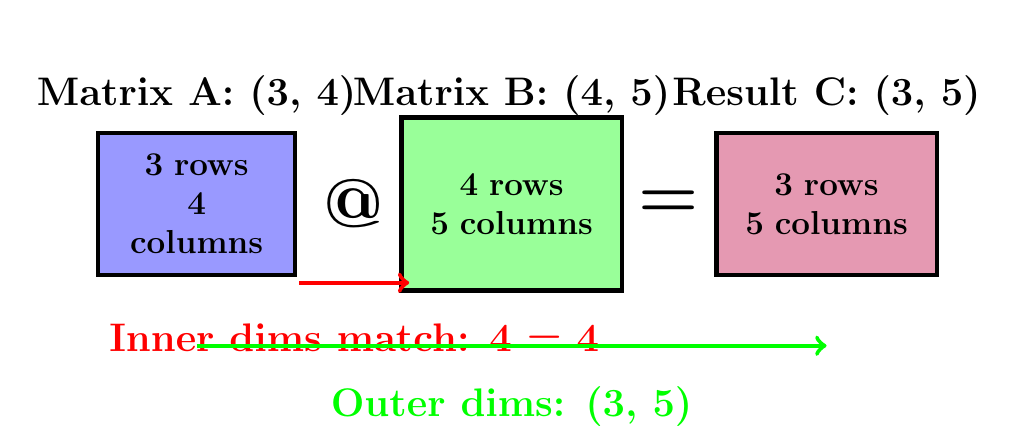
\begin{tikzpicture}[scale=1]
    % Matrix A
    \node[above, font=\Large] at (1.5, 3) {\textbf{Matrix A: (3, 4)}};
    \node[draw, ultra thick, fill=blue!40, minimum width=2.5cm, minimum height=1.8cm, text width=2cm, align=center, font=\large] at (1.5, 2) {
        \textbf{3 rows}\\
        \textbf{4 columns}
    };
    
    % @ symbol
    \node[font=\Huge] at (3.5, 2) {\textbf{@}};
    
    % Matrix B
    \node[above, font=\Large] at (5.5, 3) {\textbf{Matrix B: (4, 5)}};
    \node[draw, ultra thick, fill=green!40, minimum width=2.8cm, minimum height=2.2cm, text width=2.3cm, align=center, font=\large] at (5.5, 2) {
        \textbf{4 rows}\\
        \textbf{5 columns}
    };
    
    % = symbol
    \node[font=\Huge] at (7.5, 2) {\textbf{=}};
    
    % Result matrix C
    \node[above, font=\Large] at (9.5, 3) {\textbf{Result C: (3, 5)}};
    \node[draw, ultra thick, fill=purple!40, minimum width=2.8cm, minimum height=1.8cm, text width=2.3cm, align=center, font=\large] at (9.5, 2) {
        \textbf{3 rows}\\
        \textbf{5 columns}
    };
    
    % Dimension compatibility arrow
    \draw[ultra thick, ->, red] (2.8, 1) -- (4.2, 1);
    \node[below, red, font=\Large] at (3.5, 0.6) {\textbf{Inner dims match: 4 = 4}};
    
    % Result dimensions arrow
    \draw[ultra thick, ->, green] (1.5, 0.2) -- (9.5, 0.2);
    \node[below, green, font=\Large] at (5.5, -0.2) {\textbf{Outer dims: (3, 5)}};
\end{tikzpicture}
\end{center}

\textbf{Broadcasting in Matrix Operations:}

How PyTorch handles different dimensional operations:

\begin{center}
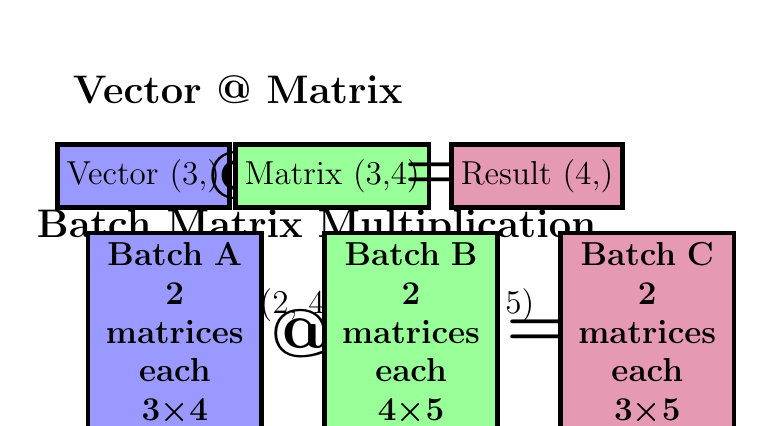
\begin{tikzpicture}[scale=1]
    % Vector @ Matrix operation (top)
    \node[above, font=\Large] at (2, 3) {\textbf{Vector @ Matrix}};
    
    \node[draw, ultra thick, fill=blue!40, minimum width=2cm, minimum height=0.8cm, font=\large] at (0.8, 2.2) {Vector (3,)};
    \node[font=\Huge] at (2, 2.2) {\textbf{@}};
    \node[draw, ultra thick, fill=green!40, minimum width=2cm, minimum height=0.8cm, font=\large] at (3.2, 2.2) {Matrix (3,4)};
    \node[font=\Huge] at (4.5, 2.2) {\textbf{=}};
    \node[draw, ultra thick, fill=purple!40, minimum width=2cm, minimum height=0.8cm, font=\large] at (5.8, 2.2) {Result (4,)};
    
    % Batch Matrix Multiplication (bottom)
    \node[above, font=\Large] at (3, 1.2) {\textbf{Batch Matrix Multiplication}};
    \node[below, font=\large] at (3, 0.9) {(2, 3, 4) @ (2, 4, 5) = (2, 3, 5)};
    
    % Batch A
    \node[draw, ultra thick, fill=blue!40, minimum width=2.2cm, minimum height=1.5cm, text width=1.8cm, align=center, font=\large] at (1.2, 0.2) {
        \textbf{Batch A}\\
        \textbf{2 matrices}\\
        \textbf{each 3×4}
    };
    
    \node[font=\Huge] at (2.8, 0.2) {\textbf{@}};
    
    % Batch B  
    \node[draw, ultra thick, fill=green!40, minimum width=2.2cm, minimum height=1.5cm, text width=1.8cm, align=center, font=\large] at (4.2, 0.2) {
        \textbf{Batch B}\\
        \textbf{2 matrices}\\
        \textbf{each 4×5}
    };
    
    \node[font=\Huge] at (5.8, 0.2) {\textbf{=}};
    
    % Batch Result
    \node[draw, ultra thick, fill=purple!40, minimum width=2.2cm, minimum height=1.5cm, text width=1.8cm, align=center, font=\large] at (7.2, 0.2) {
        \textbf{Batch C}\\
        \textbf{2 matrices}\\
        \textbf{each 3×5}
    };
\end{tikzpicture}
\end{center}

\textbf{Key Rules for Matrix Multiplication:}
\begin{itemize}
    \item \textbf{Dimension compatibility}: Inner dimensions must match (A: m×n, B: n×p → C: m×p)
    \item \textbf{Batch operations}: PyTorch handles batched matrix multiplication automatically
    \item \textbf{Broadcasting}: Vector-matrix operations broadcast appropriately
    \item \textbf{@ operator}: Preferred over torch.matmul() for readability
    \item \textbf{Memory efficiency}: Use torch.compile for optimized operations
\end{itemize}

\section{Activation Functions}

\subsection{torch.relu() and tensor.relu()}

\textbf{Purpose:} Apply Rectified Linear Unit activation function.

\textbf{Simple Example:}
\begin{minted}{python}
import torch.nn.functional as F

x = torch.tensor([-2, -1, 0, 1, 2], dtype=torch.float)

# Three ways to apply ReLU
relu1 = torch.relu(x)
relu2 = F.relu(x)
relu3 = x.relu()  # Method on tensor

print(f"Input: {x}")
# Output: Input: tensor([-2., -1.,  0.,  1.,  2.])
print(f"ReLU output: {relu1}")
# Output: ReLU output: tensor([0., 0., 0., 1., 2.])

# ReLU zeros out negative values
negative_input = torch.randn(5)
positive_output = F.relu(negative_input)
print(f"Negative input: {negative_input}")
# Output: Negative input: tensor([-0.7324,  1.2356, -0.4567,  0.8901, -1.3245])
print(f"After ReLU: {positive_output}")
# Output: After ReLU: tensor([0.0000, 1.2356, 0.0000, 0.8901, 0.0000])
\end{minted}

\textbf{Complex Example from Educational Materials:}
\begin{minted}{python}
# From micrograd Value class
def relu(self):
    out = Value(0 if self.data < 0 else self.data, (self,), 'ReLU')
    
    def _backward():
        self.grad += (out.data > 0) * out.grad
    out._backward = _backward
    return out

# From makemore generation with top-k sampling
if top_k is not None:
    v, _ = torch.topk(logits, top_k)
    # Apply ReLU-like behavior: set small values to -inf
    logits[logits < v[:, [-1]]] = -float('Inf')
\end{minted}

\subsection{torch.tanh()}

\textbf{Purpose:} Apply hyperbolic tangent activation function.

\textbf{Simple Example:}
\begin{minted}{python}
x = torch.linspace(-3, 3, 7)
tanh_output = torch.tanh(x)

print(f"Input: {x}")
# Output: Input: tensor([-3.0000, -2.0000, -1.0000,  0.0000,  1.0000,  2.0000,  3.0000])
print(f"Tanh output: {tanh_output}")
# Output: Tanh output: tensor([-0.9951, -0.9640, -0.7616,  0.0000,  0.7616,  0.9640,  0.9951])

# Tanh outputs are in range [-1, 1]
print(f"Min tanh: {tanh_output.min()}")
# Output: Min tanh: tensor(-0.9951)
print(f"Max tanh: {tanh_output.max()}")
# Output: Max tanh: tensor(0.9951)
\end{minted}

\textbf{Complex Example from Educational Materials:}
\begin{minted}{python}
# From RNN cell implementation
def forward(self, xt, hprev):
    xh = torch.cat([xt, hprev], dim=1)
    ht = F.tanh(self.xh_to_h(xh))  # Tanh activation for hidden state
    return ht

# From GRU cell
def forward(self, xt, hprev):
    # Calculate candidate hidden state
    xhr = torch.cat([xt, hprev_reset], dim=1)
    hbar = F.tanh(self.xh_to_hbar(xhr))
    
    # Blend previous and candidate states
    ht = (1 - z) * hprev + z * hbar
    return ht

# From MLP layer
self.mlpf = lambda x: m.c_proj(F.tanh(m.c_fc(x)))
\end{minted}

\chapter{Automatic Differentiation}

\section{requires\_grad and Gradient Computation}

\subsection{requires\_grad Parameter}

\textbf{Purpose:} Enable automatic gradient computation for tensors.

\textbf{Computational Graph Visualization:}

\begin{center}
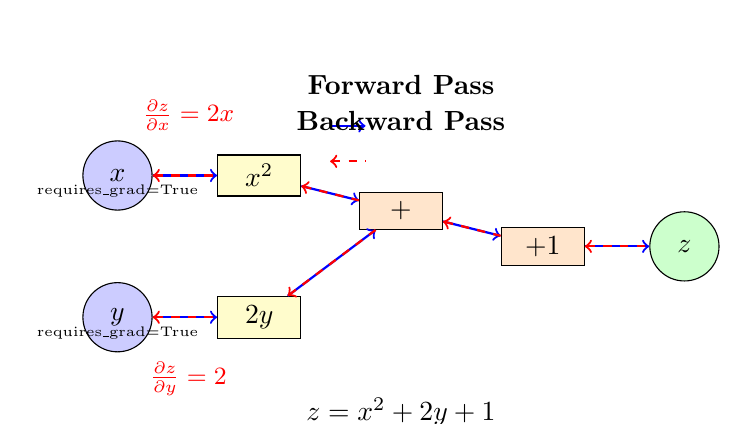
\begin{tikzpicture}[scale=0.9]
% Input nodes
\node[circle, draw, fill=blue!20, minimum size=25pt] (x) at (0,2) {$x$};
\node[circle, draw, fill=blue!20, minimum size=25pt] (y) at (0,0) {$y$};
\node[below] at (x) {\tiny requires\_grad=True};
\node[below] at (y) {\tiny requires\_grad=True};

% Operation nodes
\node[rectangle, draw, fill=yellow!20, minimum width=30pt] (pow) at (2,2) {$x^2$};
\node[rectangle, draw, fill=yellow!20, minimum width=30pt] (mul) at (2,0) {$2y$};
\node[rectangle, draw, fill=orange!20, minimum width=30pt] (add1) at (4,1.5) {$+$};
\node[rectangle, draw, fill=orange!20, minimum width=30pt] (add2) at (6,1) {$+1$};

% Output node
\node[circle, draw, fill=green!20, minimum size=25pt] (z) at (8,1) {$z$};

% Forward pass arrows
\draw[->, thick, blue] (x) -- (pow);
\draw[->, thick, blue] (y) -- (mul);
\draw[->, thick, blue] (pow) -- (add1);
\draw[->, thick, blue] (mul) -- (add1);
\draw[->, thick, blue] (add1) -- (add2);
\draw[->, thick, blue] (add2) -- (z);

% Backward pass arrows (dashed red)
\draw[<-, dashed, thick, red] (x) -- (pow);
\draw[<-, dashed, thick, red] (y) -- (mul);
\draw[<-, dashed, thick, red] (pow) -- (add1);
\draw[<-, dashed, thick, red] (mul) -- (add1);
\draw[<-, dashed, thick, red] (add1) -- (add2);
\draw[<-, dashed, thick, red] (add2) -- (z);

% Gradient values
\node[above, red] at (1,2.5) {\small $\frac{\partial z}{\partial x} = 2x$};
\node[below, red] at (1,-0.5) {\small $\frac{\partial z}{\partial y} = 2$};

% Legend
\node[above] at (4,3) {\textbf{Forward Pass}};
\draw[->, thick, blue] (3,2.7) -- (3.5,2.7);
\node[above] at (4,2.5) {\textbf{Backward Pass}};
\draw[<-, dashed, thick, red] (3,2.2) -- (3.5,2.2);

% Function definition
\node[below] at (4,-1) {$z = x^2 + 2y + 1$};
\end{tikzpicture}
\end{center}

\textbf{Simple Example:}
\begin{minted}{python}
# Create tensors that require gradients
x = torch.tensor(2.0, requires_grad=True)
y = torch.tensor(3.0, requires_grad=True)

# Perform operations
z = x**2 + 2*y + 1
print(f"z = {z}")
# Output: z = tensor(14., grad_fn=<AddBackward0>)

# Compute gradients
z.backward()
print(f"dz/dx = {x.grad}")  # Should be 2*x = 4
# Output: dz/dx = tensor(4.)
print(f"dz/dy = {y.grad}")  # Should be 2
# Output: dz/dy = tensor(2.)

# For tensors
W = torch.randn(2, 3, requires_grad=True)
print(f"W requires grad: {W.requires_grad}")
# Output: W requires grad: True
\end{minted}

\textbf{Complex Example from Educational Materials:}
\begin{minted}{python}
# From makemore neural network training
g = torch.Generator().manual_seed(2147483647)
W = torch.randn((27, 27), generator=g, requires_grad=True)

# Forward pass
xenc = F.one_hot(xs, num_classes=27).float()
logits = xenc @ W
counts = logits.exp()
probs = counts / counts.sum(1, keepdims=True)
loss = -probs[torch.arange(num), ys].log().mean() + 0.01*(W**2).mean()

# Backward pass
W.grad = None  # Clear previous gradients
loss.backward()  # Compute gradients

# Update parameters
W.data += -50 * W.grad
print(f"Gradient norm: {W.grad.norm()}")
# Output: Gradient norm: tensor(0.2847)

# PyTorch 2.x: Using autocast for mixed precision
with torch.autocast(device_type='cuda', enabled=torch.cuda.is_available()):
    logits = xenc @ W
    loss = F.cross_entropy(logits, ys)
\end{minted}

\subsection{tensor.backward()}

\textbf{Purpose:} Compute gradients using backpropagation.

\textbf{Simple Example:}
\begin{minted}{python}
# Simple function: f(x, y) = x^2 + 3xy + y^2
x = torch.tensor(1.0, requires_grad=True)
y = torch.tensor(2.0, requires_grad=True)

# Forward pass
f = x**2 + 3*x*y + y**2
print(f"Function value: {f}")
# Output: Function value: tensor(11., grad_fn=<AddBackward0>)

# Backward pass
f.backward()

print(f"df/dx: {x.grad}")  # 2x + 3y = 2(1) + 3(2) = 8
# Output: df/dx: tensor(8.)
print(f"df/dy: {y.grad}")  # 3x + 2y = 3(1) + 2(2) = 7
# Output: df/dy: tensor(7.)
\end{minted}

\textbf{Complex Example from Educational Materials:}
\begin{minted}{python}
# From makemore training loop
for step in range(max_steps):
    # Get batch
    batch = batch_loader.next()
    X, Y = [t.to(device) for t in batch]
    
    # Forward pass
    logits, loss = model(X, Y)
    
    # Backward pass
    model.zero_grad(set_to_none=True)  # Clear gradients
    loss.backward()                    # Compute gradients
    optimizer.step()                   # Update parameters
    
    if step % 10 == 0:
        print(f"step {step} | loss {loss.item():.4f}")
        # Output: step 0 | loss 2.4567

# PyTorch 2.x: Using torch.compile for optimization
model = torch.compile(model)  # Faster execution

# PyTorch 2.x: Better mixed precision training
scaler = torch.cuda.amp.GradScaler()
with torch.autocast(device_type='cuda'):
    logits, loss = model(X, Y)
    
scaler.scale(loss).backward()
scaler.step(optimizer)
scaler.update()

# From micrograd implementation
def backward(self):
    # Build topological order
    topo = []
    visited = set()
    def build_topo(v):
        if v not in visited:
            visited.add(v)
            for child in v._prev:
                build_topo(child)
            topo.append(v)
    build_topo(self)
    
    # Apply chain rule
    self.grad = 1
    for v in reversed(topo):
        v._backward()
\end{minted}

\chapter{Convolutional Neural Networks}

\section{Convolutional Layers}

\subsection{torch.nn.Conv2d}

\textbf{Purpose:} Applies 2D convolution for image processing and feature extraction.

\textbf{Syntax:} \texttt{nn.Conv2d(in\_channels, out\_channels, kernel\_size, stride=1, padding=0)}

\textbf{Convolution Operation Visualization:}

\begin{center}
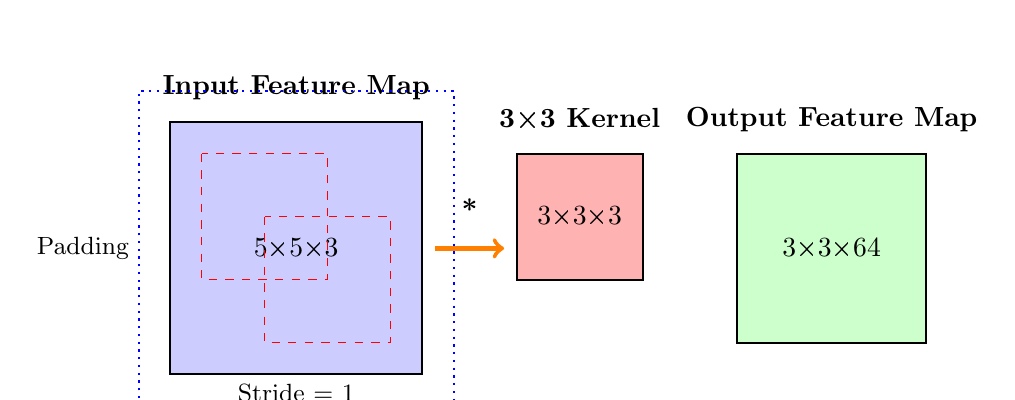
\begin{tikzpicture}[scale=0.8]
% Input feature map
\draw[thick, fill=blue!20] (0,0) rectangle (4,4);
\node[above] at (2,4.2) {\textbf{Input Feature Map}};
\node at (2,2) {5×5×3};

% Kernel/Filter
\draw[thick, fill=red!30] (5.5,1.5) rectangle (7.5,3.5);
\node[above] at (6.5,3.7) {\textbf{3×3 Kernel}};
\node at (6.5,2.5) {3×3×3};

% Convolution arrow
\draw[ultra thick, ->, orange] (4.2,2) -- (5.3,2);
\node[above] at (4.75,2.3) {\textbf{*}};

% Output feature map
\draw[thick, fill=green!20] (9,0.5) rectangle (12,3.5);
\node[above] at (10.5,3.7) {\textbf{Output Feature Map}};
\node at (10.5,2) {3×3×64};

% Stride visualization
\draw[dashed, red] (0.5,3.5) rectangle (2.5,1.5);
\draw[dashed, red] (1.5,2.5) rectangle (3.5,0.5);
\node[below] at (2,0) {\small Stride = 1};

% Padding visualization
\draw[dotted, blue, thick] (-0.5,-0.5) rectangle (4.5,4.5);
\node[left] at (-0.5,2) {\small Padding};
\end{tikzpicture}
\end{center}

\textbf{Simple Example:}
\begin{minted}{python}
import torch.nn as nn

# Basic convolution layer
conv = nn.Conv2d(
    in_channels=3,      # RGB input
    out_channels=64,    # 64 feature maps
    kernel_size=3,      # 3x3 kernel
    stride=1,          # Stride of 1
    padding=1          # Padding to keep size
)

# Input: batch_size=32, channels=3, height=224, width=224
x = torch.randn(32, 3, 224, 224)
output = conv(x)
print(f"Input shape: {x.shape}")     # torch.Size([32, 3, 224, 224])
print(f"Output shape: {output.shape}") # torch.Size([32, 64, 224, 224])

# Access layer parameters
print(f"Weight shape: {conv.weight.shape}")  # torch.Size([64, 3, 3, 3])
print(f"Bias shape: {conv.bias.shape}")      # torch.Size([64])
\end{minted}

\textbf{Complex Example - CNN Architecture:}
\begin{minted}{python}
class CNN_Classifier(nn.Module):
    def __init__(self, num_classes=10):
        super().__init__()
        
        # Feature extraction layers
        self.features = nn.Sequential(
            # First conv block
            nn.Conv2d(3, 64, kernel_size=3, padding=1),
            nn.BatchNorm2d(64),
            nn.ReLU(inplace=True),
            nn.MaxPool2d(kernel_size=2, stride=2),
            
            # Second conv block
            nn.Conv2d(64, 128, kernel_size=3, padding=1),
            nn.BatchNorm2d(128),
            nn.ReLU(inplace=True),
            nn.MaxPool2d(kernel_size=2, stride=2),
            
            # Third conv block
            nn.Conv2d(128, 256, kernel_size=3, padding=1),
            nn.BatchNorm2d(256),
            nn.ReLU(inplace=True),
            nn.MaxPool2d(kernel_size=2, stride=2),
        )
        
        # Classifier
        self.classifier = nn.Sequential(
            nn.AdaptiveAvgPool2d((7, 7)),
            nn.Flatten(),
            nn.Linear(256 * 7 * 7, 512),
            nn.ReLU(inplace=True),
            nn.Dropout(0.5),
            nn.Linear(512, num_classes)
        )
    
    def forward(self, x):
        x = self.features(x)
        x = self.classifier(x)
        return x

# Usage
model = CNN_Classifier(num_classes=1000)
input_tensor = torch.randn(16, 3, 224, 224)
output = model(input_tensor)
print(f"Output shape: {output.shape}")  # torch.Size([16, 1000])
\end{minted}

\textbf{CNN Architecture Visualization:}

\begin{center}
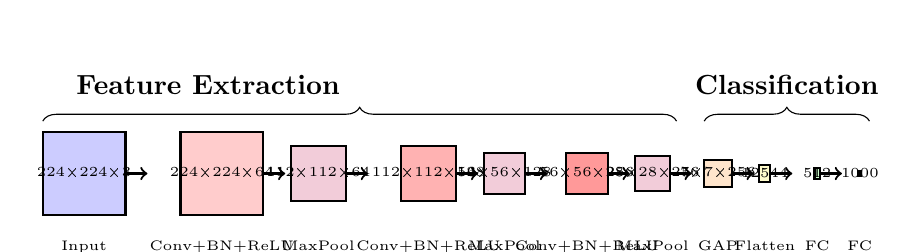
\begin{tikzpicture}[scale=0.7]
% Input
\draw[thick, fill=blue!20] (0,0) rectangle (1.5,1.5);
\node[below] at (0.75,-0.3) {\tiny Input};
\node at (0.75,0.75) {\tiny 224×224×3};

% First conv block
\draw[thick, fill=red!20] (2.5,0) rectangle (4,1.5);
\node[below] at (3.25,-0.3) {\tiny Conv+BN+ReLU};
\node at (3.25,0.75) {\tiny 224×224×64};

\draw[thick, fill=purple!20] (4.5,0.25) rectangle (5.5,1.25);
\node[below] at (5,-0.3) {\tiny MaxPool};
\node at (5,0.75) {\tiny 112×112×64};

% Second conv block
\draw[thick, fill=red!30] (6.5,0.25) rectangle (7.5,1.25);
\node[below] at (7,-0.3) {\tiny Conv+BN+ReLU};
\node at (7,0.75) {\tiny 112×112×128};

\draw[thick, fill=purple!20] (8,0.375) rectangle (8.75,1.125);
\node[below] at (8.375,-0.3) {\tiny MaxPool};
\node at (8.375,0.75) {\tiny 56×56×128};

% Third conv block
\draw[thick, fill=red!40] (9.5,0.375) rectangle (10.25,1.125);
\node[below] at (9.875,-0.3) {\tiny Conv+BN+ReLU};
\node at (9.875,0.75) {\tiny 56×56×256};

\draw[thick, fill=purple!20] (10.75,0.4375) rectangle (11.375,1.0625);
\node[below] at (11.0625,-0.3) {\tiny MaxPool};
\node at (11.0625,0.75) {\tiny 28×28×256};

% Global Average Pooling
\draw[thick, fill=orange!20] (12,0.5) rectangle (12.5,1);
\node[below] at (12.25,-0.3) {\tiny GAP};
\node at (12.25,0.75) {\tiny 7×7×256};

% Flatten
\draw[thick, fill=yellow!20] (13,0.6) rectangle (13.2,0.9);
\node[below] at (13.1,-0.3) {\tiny Flatten};
\node at (13.1,0.75) {\tiny 12544};

% FC layers
\draw[thick, fill=green!20] (14,0.65) rectangle (14.1,0.85);
\node[below] at (14.05,-0.3) {\tiny FC};
\node at (14.05,0.75) {\tiny 512};

\draw[thick, fill=green!30] (14.8,0.7) rectangle (14.85,0.8);
\node[below] at (14.825,-0.3) {\tiny FC};
\node at (14.825,0.75) {\tiny 1000};

% Arrows
\foreach \x in {1.5,4,5.5,7.5,8.75,10.25,11.375,12.5,13.2,14.1} {
    \draw[->, thick] (\x,0.75) -- (\x+0.4,0.75);
}

% Labels for feature reduction
\node[above] at (3,2) {\textbf{Feature Extraction}};
\node[above] at (13.5,2) {\textbf{Classification}};
\draw[decorate, decoration={brace, amplitude=5pt}] (0,1.7) -- (11.5,1.7);
\draw[decorate, decoration={brace, amplitude=5pt}] (12,1.7) -- (15,1.7);
\end{tikzpicture}
\end{center}

\section{Pooling Layers}

\subsection{torch.nn.MaxPool2d}

\textbf{Purpose:} Applies max pooling for downsampling and translation invariance.

\textbf{Max Pooling Operation Visualization:}

\begin{center}
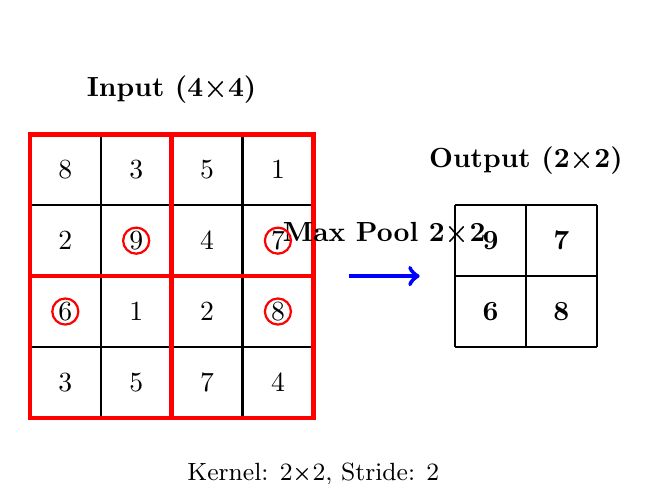
\begin{tikzpicture}[scale=0.9]
% Input feature map (4x4)
\draw[thick] (0,0) grid (4,4);
\foreach \x/\y/\val in {0/3/8, 1/3/3, 2/3/5, 3/3/1, 0/2/2, 1/2/9, 2/2/4, 3/2/7, 0/1/6, 1/1/1, 2/1/2, 3/1/8, 0/0/3, 1/0/5, 2/0/7, 3/0/4} {
    \node at (\x+0.5,\y+0.5) {\val};
}
\node[above] at (2,4.3) {\textbf{Input (4×4)}};

% Pooling windows
\draw[red, ultra thick] (0,2) rectangle (2,4);
\draw[red, ultra thick] (2,2) rectangle (4,4);
\draw[red, ultra thick] (0,0) rectangle (2,2);
\draw[red, ultra thick] (2,0) rectangle (4,2);

% Arrow
\draw[ultra thick, ->, blue] (4.5,2) -- (5.5,2);
\node[above] at (5,2.3) {\textbf{Max Pool 2×2}};

% Output feature map (2x2)
\draw[thick] (6,1) grid (8,3);
\node at (6.5,2.5) {\textbf{9}};
\node at (7.5,2.5) {\textbf{7}};
\node at (6.5,1.5) {\textbf{6}};
\node at (7.5,1.5) {\textbf{8}};
\node[above] at (7,3.3) {\textbf{Output (2×2)}};

% Max values highlighted
\node[circle, draw=red, thick] at (1.5,2.5) {};
\node[circle, draw=red, thick] at (3.5,2.5) {};
\node[circle, draw=red, thick] at (0.5,1.5) {};
\node[circle, draw=red, thick] at (3.5,1.5) {};

% Pooling operation details
\node[below] at (4,-0.5) {\small Kernel: 2×2, Stride: 2};
\end{tikzpicture}
\end{center}

\textbf{Simple Example:}
\begin{minted}{python}
# Max pooling layer
maxpool = nn.MaxPool2d(
    kernel_size=2,    # 2x2 pooling window
    stride=2,        # Non-overlapping windows
    padding=0        # No padding
)

# Input: 64 feature maps of size 56x56
x = torch.randn(32, 64, 56, 56)
output = maxpool(x)
print(f"Input shape: {x.shape}")     # torch.Size([32, 64, 56, 56])
print(f"Output shape: {output.shape}") # torch.Size([32, 64, 28, 28])

# Average pooling
avgpool = nn.AvgPool2d(kernel_size=2, stride=2)
avg_output = avgpool(x)
print(f"AvgPool output: {avg_output.shape}")  # torch.Size([32, 64, 28, 28])
\end{minted}

\textbf{Complex Example - Adaptive Pooling:}
\begin{minted}{python}
# Adaptive pooling - always produces fixed output size
adaptive_avg = nn.AdaptiveAvgPool2d((7, 7))  # Always 7x7 output
adaptive_max = nn.AdaptiveMaxPool2d((1, 1))  # Global pooling

# Different input sizes
inputs = [
    torch.randn(1, 256, 14, 14),  # Small feature map
    torch.randn(1, 256, 28, 28),  # Medium feature map
    torch.randn(1, 256, 56, 56),  # Large feature map
]

for i, input_tensor in enumerate(inputs):
    # Adaptive average pooling
    avg_out = adaptive_avg(input_tensor)
    max_out = adaptive_max(input_tensor)
    
    print(f"Input {i+1}: {input_tensor.shape}")
    print(f"  Adaptive Avg: {avg_out.shape}")      # Always (1, 256, 7, 7)
    print(f"  Adaptive Max: {max_out.shape}")      # Always (1, 256, 1, 1)

# Global Average Pooling (common in modern architectures)
class GlobalAvgPool(nn.Module):
    def forward(self, x):
        # x: (batch_size, channels, height, width)
        return F.adaptive_avg_pool2d(x, (1, 1)).view(x.size(0), -1)

gap = GlobalAvgPool()
x = torch.randn(32, 512, 7, 7)
output = gap(x)
print(f"Global pooling output: {output.shape}")  # torch.Size([32, 512])
\end{minted}

\section{Activation Functions}

\subsection{torch.nn.GELU}

\textbf{Purpose:} Gaussian Error Linear Unit - modern activation function used in transformers.

\textbf{Simple Example:}
\begin{minted}{python}
# GELU activation (used in BERT, GPT)
gelu = nn.GELU()
x = torch.randn(5)
output = gelu(x)

print(f"Input: {x}")
# Output: Input: tensor([-2.0000, -1.0000,  0.0000,  1.0000,  2.0000])
print(f"GELU output: {output}")
# Output: GELU output: tensor([-0.0455, -0.1588,  0.0000,  0.8413,  1.9545])

# Compare with ReLU
relu = nn.ReLU()
relu_output = relu(x)
print(f"ReLU output: {relu_output}")
# Output: ReLU output: tensor([0.0000, 0.0000, 0.0000, 1.0000, 2.0000])

# GELU is smoother than ReLU, allowing small negative values
\end{minted}

\textbf{Complex Example - Modern Activation Functions:}
\begin{minted}{python}
# Comparison of modern activation functions
activations = {
    'ReLU': nn.ReLU(),
    'GELU': nn.GELU(),
    'SiLU (Swish)': nn.SiLU(),
    'Mish': nn.Mish(),
    'LeakyReLU': nn.LeakyReLU(0.1)
}

x = torch.linspace(-3, 3, 100)

# Test all activations
for name, activation in activations.items():
    y = activation(x)
    print(f"{name}: min={y.min():.3f}, max={y.max():.3f}")
    # Output: ReLU: min=0.000, max=2.000
    # Output: GELU: min=-0.046, max=1.955
    # Output: Tanh: min=-0.995, max=0.995

# Modern MLP with GELU
class ModernMLP(nn.Module):
    def __init__(self, input_dim, hidden_dim, output_dim):
        super().__init__()
        self.layers = nn.Sequential(
            nn.Linear(input_dim, hidden_dim),
            nn.GELU(),                          # Modern activation
            nn.LayerNorm(hidden_dim),           # Layer normalization
            nn.Dropout(0.1),
            nn.Linear(hidden_dim, hidden_dim),
            nn.GELU(),
            nn.LayerNorm(hidden_dim),
            nn.Dropout(0.1),
            nn.Linear(hidden_dim, output_dim)
        )
    
    def forward(self, x):
        return self.layers(x)
\end{minted}

\chapter{Neural Network Building Blocks}

\section{Linear Layers}

\subsection{torch.nn.Linear}

\textbf{Purpose:} Applies a linear transformation: $y = xW^T + b$.

\textbf{Neural Network Architecture Visualization:}

\begin{center}
\begin{tikzpicture}[scale=0.8]
% Input layer
\foreach \y in {1,2,3,4,5} {
    \node[circle, draw, fill=blue!20, minimum size=20pt] (I\y) at (0,\y) {$x_{\y}$};
}
\node[above] at (0,5.5) {\textbf{Input Layer}};
\node[below] at (0,0.5) {\small (5 features)};

% Hidden layer 1
\foreach \y in {1.5,2.5,3.5,4.5} {
    \node[circle, draw, fill=red!20, minimum size=20pt] (H1\y) at (3,\y) {};
}
\node[above] at (3,5) {\textbf{Hidden Layer 1}};
\node[below] at (3,1) {\small (4 units)};

% Hidden layer 2
\foreach \y in {2,3,4} {
    \node[circle, draw, fill=orange!20, minimum size=20pt] (H2\y) at (6,\y) {};
}
\node[above] at (6,4.5) {\textbf{Hidden Layer 2}};
\node[below] at (6,1.5) {\small (3 units)};

% Output layer
\foreach \y in {2.5,3.5} {
    \node[circle, draw, fill=green!20, minimum size=20pt] (O\y) at (9,\y) {$y_{\y}$};
}
\node[above] at (9,4) {\textbf{Output Layer}};
\node[below] at (9,2) {\small (2 classes)};

% Connections from input to hidden1
\foreach \i in {1,2,3,4,5} {
    \foreach \j in {1.5,2.5,3.5,4.5} {
        \draw[->, thin, gray] (I\i) -- (H1\j);
    }
}

% Connections from hidden1 to hidden2
\foreach \i in {1.5,2.5,3.5,4.5} {
    \foreach \j in {2,3,4} {
        \draw[->, thin, gray] (H1\i) -- (H2\j);
    }
}

% Connections from hidden2 to output
\foreach \i in {2,3,4} {
    \foreach \j in {2.5,3.5} {
        \draw[->, thin, gray] (H2\i) -- (O\j);
    }
}

% Linear transformation labels
\node[above, rotate=15] at (1.5,3.5) {\small $W_1, b_1$};
\node[above, rotate=15] at (4.5,3.2) {\small $W_2, b_2$};
\node[above, rotate=15] at (7.5,3) {\small $W_3, b_3$};

% Activation functions
\node[below, fill=white, draw, rounded corners] at (3,0.5) {\small ReLU};
\node[below, fill=white, draw, rounded corners] at (6,1) {\small ReLU};
\node[below, fill=white, draw, rounded corners] at (9,1.5) {\small Softmax};
\end{tikzpicture}
\end{center}

\textbf{Simple Example:}
\begin{minted}{python}
import torch.nn as nn

# Create a linear layer
linear = nn.Linear(in_features=5, out_features=3)
print(f"Weight shape: {linear.weight.shape}")  # (3, 5)
# Output: Weight shape: torch.Size([3, 5])
print(f"Bias shape: {linear.bias.shape}")      # (3,)
# Output: Bias shape: torch.Size([3])

# Forward pass
x = torch.randn(2, 5)  # Batch of 2 samples, 5 features each
y = linear(x)
print(f"Input shape: {x.shape}")   # (2, 5)
# Output: Input shape: torch.Size([2, 5])
print(f"Output shape: {y.shape}")  # (2, 3)
# Output: Output shape: torch.Size([2, 3])

# PyTorch 2.x: Using device and dtype initialization
device = "cuda" if torch.cuda.is_available() else "cpu"
linear_gpu = nn.Linear(5, 3, device=device, dtype=torch.float16)
print(f"Layer on {device} with dtype {linear_gpu.weight.dtype}")
# Output: Layer on cpu with dtype torch.float32
\end{minted}

\textbf{Complex Example from Educational Materials:}
\begin{minted}{python}
# From Transformer implementation
class CausalSelfAttention(nn.Module):
    def __init__(self, config):
        super().__init__()
        # Key, query, value projections for all heads
        self.c_attn = nn.Linear(config.n_embd, 3 * config.n_embd)
        # Output projection
        self.c_proj = nn.Linear(config.n_embd, config.n_embd)
    
    def forward(self, x):
        # Apply linear transformations
        q, k, v = self.c_attn(x).split(self.n_embd, dim=2)
        y = self.c_proj(y)
        return y

# From MLP implementation
class MLP(nn.Module):
    def __init__(self, config):
        super().__init__()
        self.mlp = nn.Sequential(
            nn.Linear(self.block_size * config.n_embd, config.n_embd2),
            nn.Tanh(),
            nn.Linear(config.n_embd2, self.vocab_size)
        )
\end{minted}

\section{Embedding Layers}

\subsection{torch.nn.Embedding}

\textbf{Purpose:} Creates learnable lookup tables for discrete tokens.

\textbf{Simple Example:}
\begin{minted}{python}
# Create embedding layer
vocab_size = 1000
embedding_dim = 128
embedding = nn.Embedding(vocab_size, embedding_dim)

# Input: token indices
tokens = torch.tensor([1, 5, 23, 100])
embedded = embedding(tokens)

print(f"Token indices: {tokens}")
# Output: Token indices: tensor([  1,   5,  23, 100])
print(f"Embedded shape: {embedded.shape}")  # (4, 128)
# Output: Embedded shape: torch.Size([4, 128])
print(f"Each token -> {embedding_dim}D vector")
# Output: Each token -> 128D vector

# Batch processing
batch_tokens = torch.tensor([[1, 5, 23], [45, 67, 89]])
batch_embedded = embedding(batch_tokens)
print(f"Batch embedded shape: {batch_embedded.shape}")  # (2, 3, 128)
# Output: Batch embedded shape: torch.Size([2, 3, 128])
\end{minted}

\textbf{Complex Example from Educational Materials:}
\begin{minted}{python}
# From Transformer language model
class Transformer(nn.Module):
    def __init__(self, config):
        super().__init__()
        self.transformer = nn.ModuleDict(dict(
            wte = nn.Embedding(config.vocab_size, config.n_embd),    # Token embeddings
            wpe = nn.Embedding(config.block_size, config.n_embd),    # Position embeddings
            h = nn.ModuleList([Block(config) for _ in range(config.n_layer)]),
            ln_f = nn.LayerNorm(config.n_embd),
        ))
    
    def forward(self, idx, targets=None):
        b, t = idx.size()
        pos = torch.arange(0, t, dtype=torch.long, device=device).unsqueeze(0)
        
        # Get embeddings
        tok_emb = self.transformer.wte(idx)  # Token embeddings
        pos_emb = self.transformer.wpe(pos)  # Position embeddings
        x = tok_emb + pos_emb  # Combine both
        
        return x

# From MLP model
self.wte = nn.Embedding(config.vocab_size + 1, config.n_embd)
# +1 for special <BLANK> token
\end{minted}

\section{Normalization Layers}

\subsection{torch.nn.Dropout}

\textbf{Purpose:} Applies dropout regularization to prevent overfitting.

\textbf{Simple Example:}
\begin{minted}{python}
# Dropout layer
dropout = nn.Dropout(p=0.5)  # Drop 50% of neurons during training

# Input tensor
x = torch.randn(32, 128)
print(f"Input: {x[0, :10]}")  # First 10 values of first sample
# Output: Input: tensor([ 0.7342, -1.2456,  0.9876, -0.3421,  1.5643, -0.8765,  0.2134, -1.6789,  0.4321, -0.7654])

# During training (dropout active)
model.train()
dropped = dropout(x)
print(f"Dropped: {dropped[0, :10]}")  # Some values are zero
# Output: Dropped: tensor([ 1.4684,  0.0000,  1.9752, -0.6842,  0.0000, -1.7530,  0.4268,  0.0000,  0.8642,  0.0000])

# During evaluation (dropout inactive)
model.eval()
eval_output = dropout(x)
print(f"Eval: {eval_output[0, :10]}")  # All values preserved
# Output: Eval: tensor([ 0.7342, -1.2456,  0.9876, -0.3421,  1.5643, -0.8765,  0.2134, -1.6789,  0.4321, -0.7654])
\end{minted}

\textbf{Complex Example - Different Dropout Types:}
\begin{minted}{python}
class DropoutComparison(nn.Module):
    def __init__(self):
        super().__init__()
        # Standard dropout
        self.dropout = nn.Dropout(0.3)
        
        # Dropout for convolutional layers
        self.dropout2d = nn.Dropout2d(0.25)  # Drops entire feature maps
        
        # Alpha dropout (for SELU activation)
        self.alpha_dropout = nn.AlphaDropout(0.3)
        
        # Feature alpha dropout
        self.feature_alpha_dropout = nn.FeatureAlphaDropout(0.3)
    
    def forward(self, x_linear, x_conv):
        # Linear layer dropout
        x_linear = self.dropout(x_linear)
        
        # Convolutional dropout (drops entire channels)
        x_conv = self.dropout2d(x_conv)
        
        return x_linear, x_conv

# Example usage in CNN
class RegularizedCNN(nn.Module):
    def __init__(self, num_classes):
        super().__init__()
        self.features = nn.Sequential(
            nn.Conv2d(3, 64, 3, padding=1),
            nn.ReLU(),
            nn.Dropout2d(0.1),  # Spatial dropout
            
            nn.Conv2d(64, 128, 3, padding=1),
            nn.ReLU(),
            nn.MaxPool2d(2),
            nn.Dropout2d(0.2),
        )
        
        self.classifier = nn.Sequential(
            nn.Linear(128 * 14 * 14, 512),
            nn.ReLU(),
            nn.Dropout(0.5),  # Standard dropout
            nn.Linear(512, num_classes)
        )
    
    def forward(self, x):
        x = self.features(x)
        x = x.view(x.size(0), -1)
        x = self.classifier(x)
        return x
\end{minted}

\subsection{torch.nn.BatchNorm2d}

\textbf{Purpose:} Applies batch normalization for faster training and regularization.

\textbf{Simple Example:}
\begin{minted}{python}
# Batch normalization for 2D inputs (after Conv2d)
batch_norm = nn.BatchNorm2d(64)  # 64 feature channels

# Input: (batch_size, channels, height, width)
x = torch.randn(32, 64, 28, 28)
normalized = batch_norm(x)

print(f"Input shape: {x.shape}")
# Output: Input shape: torch.Size([32, 64, 28, 28])
print(f"Output shape: {normalized.shape}")
# Output: Output shape: torch.Size([32, 64, 28, 28])

# Check statistics
print(f"Mean per channel: {normalized.mean(dim=[0,2,3])}")  # Should be ~0
# Output: Mean per channel: tensor([-0.0012,  0.0023, -0.0045, ...,  0.0018])
print(f"Std per channel: {normalized.std(dim=[0,2,3])}")    # Should be ~1
# Output: Std per channel: tensor([0.9987, 1.0034, 0.9956, ..., 1.0012])

# Access learned parameters
print(f"Gamma (scale): {batch_norm.weight.shape}")  # (64,)
# Output: Gamma (scale): torch.Size([64])
print(f"Beta (shift): {batch_norm.bias.shape}")     # (64,)
# Output: Beta (shift): torch.Size([64])
\end{minted}

\textbf{Complex Example - Normalization Comparison:}
\begin{minted}{python}
class NormalizationComparison(nn.Module):
    def __init__(self, channels, height, width):
        super().__init__()
        # Different normalization techniques
        self.batch_norm = nn.BatchNorm2d(channels)
        self.layer_norm = nn.LayerNorm([channels, height, width])
        self.instance_norm = nn.InstanceNorm2d(channels)
        self.group_norm = nn.GroupNorm(8, channels)  # 8 groups
        
    def forward(self, x):
        # x shape: (batch, channels, height, width)
        
        # Batch normalization: normalize across batch dimension
        bn_out = self.batch_norm(x)
        
        # Layer normalization: normalize across channel, height, width
        ln_out = self.layer_norm(x)
        
        # Instance normalization: normalize per instance per channel
        in_out = self.instance_norm(x)
        
        # Group normalization: normalize within groups of channels
        gn_out = self.group_norm(x)
        
        return {
            'batch_norm': bn_out,
            'layer_norm': ln_out,
            'instance_norm': in_out,
            'group_norm': gn_out
        }

# Modern CNN block with proper normalization
class ModernConvBlock(nn.Module):
    def __init__(self, in_channels, out_channels, use_residual=False):
        super().__init__()
        self.use_residual = use_residual
        
        self.conv1 = nn.Conv2d(in_channels, out_channels, 3, padding=1, bias=False)
        self.bn1 = nn.BatchNorm2d(out_channels)
        self.conv2 = nn.Conv2d(out_channels, out_channels, 3, padding=1, bias=False)
        self.bn2 = nn.BatchNorm2d(out_channels)
        
        # Residual connection
        if use_residual and in_channels != out_channels:
            self.residual = nn.Conv2d(in_channels, out_channels, 1, bias=False)
        else:
            self.residual = nn.Identity()
    
    def forward(self, x):
        identity = x
        
        out = F.relu(self.bn1(self.conv1(x)))
        out = self.bn2(self.conv2(out))
        
        if self.use_residual:
            out += self.residual(identity)
        
        return F.relu(out)
\end{minted}

\subsection{torch.nn.LayerNorm}

\textbf{Purpose:} Applies layer normalization to stabilize training.

\textbf{Simple Example:}
\begin{minted}{python}
# Create layer norm
layer_norm = nn.LayerNorm(4)  # Normalize over last dimension

# Input tensor
x = torch.randn(2, 3, 4)  # (batch, sequence, features)
normalized = layer_norm(x)

print(f"Input shape: {x.shape}")
# Output: Input shape: torch.Size([2, 3, 4])
print(f"Output shape: {normalized.shape}")
# Output: Output shape: torch.Size([2, 3, 4])

# Check normalization: mean approximately 0, std approximately 1 for last dimension
print(f"Mean along last dim: {normalized.mean(dim=-1)}")
# Output: Mean along last dim: tensor([[-0.0000, -0.0000,  0.0000],
#                                     [ 0.0000,  0.0000, -0.0000]])
print(f"Std along last dim: {normalized.std(dim=-1)}")
# Output: Std along last dim: tensor([[1.0000, 1.0000, 1.0000],
#                                    [1.0000, 1.0000, 1.0000]])
\end{minted}

\textbf{Complex Example from Educational Materials:}
\begin{minted}{python}
# From Transformer block
class Block(nn.Module):
    def __init__(self, config):
        super().__init__()
        self.ln_1 = nn.LayerNorm(config.n_embd)  # Pre-attention norm
        self.attn = CausalSelfAttention(config)
        self.ln_2 = nn.LayerNorm(config.n_embd)  # Pre-MLP norm
        self.mlp = nn.ModuleDict(dict(
            c_fc    = nn.Linear(config.n_embd, 4 * config.n_embd),
            c_proj  = nn.Linear(4 * config.n_embd, config.n_embd),
            act     = NewGELU(),
        ))
    
    def forward(self, x):
        # Pre-norm architecture
        x = x + self.attn(self.ln_1(x))     # Residual + attention
        x = x + self.mlpf(self.ln_2(x))     # Residual + MLP
        return x

# Final layer norm before output
self.transformer = nn.ModuleDict(dict(
    wte = nn.Embedding(config.vocab_size, config.n_embd),
    wpe = nn.Embedding(config.block_size, config.n_embd),
    h = nn.ModuleList([Block(config) for _ in range(config.n_layer)]),
    ln_f = nn.LayerNorm(config.n_embd),  # Final layer norm
))
\end{minted}

\chapter{Essential Deep Learning Utilities}

\section{Gradient Clipping}

\subsection{torch.nn.utils.clip\_grad\_norm\_()}

\textbf{Purpose:} Clips gradient norm of parameters to prevent gradient explosion.

\textbf{Syntax:} \texttt{torch.nn.utils.clip\_grad\_norm\_(parameters, max\_norm, norm\_type=2.0)}

\textbf{Simple Example:}
\begin{minted}{python}
import torch
import torch.nn as nn
import torch.nn.utils as utils

# Simple model
model = nn.Sequential(
    nn.Linear(10, 50),
    nn.ReLU(),
    nn.Linear(50, 1)
)

# Training step with gradient clipping
optimizer = torch.optim.Adam(model.parameters(), lr=0.001)
criterion = nn.MSELoss()

x = torch.randn(32, 10)
y = torch.randn(32, 1)

# Forward pass
output = model(x)
loss = criterion(output, y)

# Backward pass with gradient clipping
optimizer.zero_grad()
loss.backward()

# Clip gradients before optimizer step
grad_norm = utils.clip_grad_norm_(model.parameters(), max_norm=1.0)
print(f"Gradient norm before clipping: {grad_norm}")
# Output: Gradient norm before clipping: tensor(2.4567)

optimizer.step()
\end{minted}

\textbf{Complex Example - RNN Training:}
\begin{minted}{python}
# Training loop with gradient clipping for RNN
class LSTM_Model(nn.Module):
    def __init__(self, vocab_size, embed_size, hidden_size, num_layers):
        super().__init__()
        self.embedding = nn.Embedding(vocab_size, embed_size)
        self.lstm = nn.LSTM(embed_size, hidden_size, num_layers, batch_first=True)
        self.fc = nn.Linear(hidden_size, vocab_size)
        
    def forward(self, x, hidden=None):
        embedded = self.embedding(x)
        lstm_out, hidden = self.lstm(embedded, hidden)
        output = self.fc(lstm_out)
        return output, hidden

model = LSTM_Model(vocab_size=10000, embed_size=256, hidden_size=512, num_layers=2)
optimizer = torch.optim.Adam(model.parameters(), lr=0.001)

for epoch in range(num_epochs):
    for batch in dataloader:
        input_ids, target_ids = batch
        
        # Forward pass
        output, _ = model(input_ids)
        loss = F.cross_entropy(output.view(-1, vocab_size), target_ids.view(-1))
        
        # Backward pass with gradient clipping
        optimizer.zero_grad()
        loss.backward()
        
        # Essential for RNN training - prevents exploding gradients
        torch.nn.utils.clip_grad_norm_(model.parameters(), max_norm=0.5)
        
        optimizer.step()
\end{minted}

\subsection{torch.nn.utils.clip\_grad\_value\_()}

\textbf{Purpose:} Clips gradients at a specified value.

\textbf{Simple Example:}
\begin{minted}{python}
# Value-based gradient clipping
optimizer.zero_grad()
loss.backward()

# Clip individual gradient values to [-0.5, 0.5]
torch.nn.utils.clip_grad_value_(model.parameters(), clip_value=0.5)

optimizer.step()
\end{minted}

\section{Model Utilities}

\subsection{torch.save() and torch.load()}

\textbf{Purpose:} Save and load models, optimizers, and training state.

\textbf{Simple Example:}
\begin{minted}{python}
# Save model state dict (recommended)
torch.save(model.state_dict(), 'model_weights.pth')

# Load model state dict
model = MyModel()
model.load_state_dict(torch.load('model_weights.pth'))
model.eval()

# Save entire model (less flexible)
torch.save(model, 'complete_model.pth')
loaded_model = torch.load('complete_model.pth')
\end{minted}

\textbf{Complex Example - Training Checkpoint:}
\begin{minted}{python}
# Save complete training state
def save_checkpoint(model, optimizer, scheduler, epoch, loss, filepath):
    checkpoint = {
        'epoch': epoch,
        'model_state_dict': model.state_dict(),
        'optimizer_state_dict': optimizer.state_dict(),
        'scheduler_state_dict': scheduler.state_dict(),
        'loss': loss,
        'model_config': model.config  # Save model configuration
    }
    torch.save(checkpoint, filepath)

# Load complete training state
def load_checkpoint(filepath, model, optimizer=None, scheduler=None):
    checkpoint = torch.load(filepath, map_location='cpu')
    
    model.load_state_dict(checkpoint['model_state_dict'])
    
    if optimizer:
        optimizer.load_state_dict(checkpoint['optimizer_state_dict'])
    
    if scheduler:
        scheduler.load_state_dict(checkpoint['scheduler_state_dict'])
    
    return checkpoint['epoch'], checkpoint['loss']

# Usage in training loop
if epoch % save_interval == 0:
    save_checkpoint(model, optimizer, scheduler, epoch, loss, 
                   f'checkpoint_epoch_{epoch}.pth')

# Resume training
epoch_start, prev_loss = load_checkpoint('checkpoint_epoch_100.pth', 
                                        model, optimizer, scheduler)
\end{minted}

\section{Parameter Initialization}

\subsection{torch.nn.init Functions}

\textbf{Purpose:} Initialize model parameters with specific distributions.

\textbf{Simple Example:}
\begin{minted}{python}
import torch.nn.init as init

# Initialize a linear layer
layer = nn.Linear(100, 50)

# Xavier/Glorot initialization
init.xavier_uniform_(layer.weight)
init.zeros_(layer.bias)

# Kaiming/He initialization (good for ReLU)
init.kaiming_normal_(layer.weight, mode='fan_out', nonlinearity='relu')

# Normal initialization
init.normal_(layer.weight, mean=0, std=0.01)

# Constant initialization
init.constant_(layer.bias, 0)
\end{minted}

\textbf{Complex Example - Custom Model Initialization:}
\begin{minted}{python}
class CustomCNN(nn.Module):
    def __init__(self, num_classes):
        super().__init__()
        self.conv1 = nn.Conv2d(3, 64, kernel_size=3, padding=1)
        self.conv2 = nn.Conv2d(64, 128, kernel_size=3, padding=1)
        self.fc1 = nn.Linear(128 * 8 * 8, 512)
        self.fc2 = nn.Linear(512, num_classes)
        
        # Custom initialization
        self._initialize_weights()
    
    def _initialize_weights(self):
        for module in self.modules():
            if isinstance(module, nn.Conv2d):
                # Kaiming initialization for conv layers
                nn.init.kaiming_normal_(module.weight, mode='fan_out', 
                                      nonlinearity='relu')
                if module.bias is not None:
                    nn.init.constant_(module.bias, 0)
            elif isinstance(module, nn.Linear):
                # Xavier initialization for linear layers
                nn.init.xavier_normal_(module.weight)
                nn.init.constant_(module.bias, 0)

# Alternative: Initialize after model creation
def init_weights(module):
    if isinstance(module, nn.Linear):
        torch.nn.init.xavier_uniform_(module.weight)
        module.bias.data.fill_(0.01)
    elif isinstance(module, nn.Conv2d):
        torch.nn.init.kaiming_uniform_(module.weight)

model = CustomCNN(num_classes=10)
model.apply(init_weights)  # Apply to all modules
\end{minted}

\section{Data Utilities}

\subsection{torch.utils.data.DataLoader}

\textbf{Purpose:} Efficient data loading with batching, shuffling, and multiprocessing.

\textbf{Simple Example:}
\begin{minted}{python}
from torch.utils.data import DataLoader, TensorDataset

# Create dataset
x_data = torch.randn(1000, 10)
y_data = torch.randn(1000, 1)
dataset = TensorDataset(x_data, y_data)

# Create dataloader
dataloader = DataLoader(
    dataset,
    batch_size=32,
    shuffle=True,
    num_workers=4,
    pin_memory=True  # Faster GPU transfer
)

# Training loop
for batch_idx, (data, targets) in enumerate(dataloader):
    # Move to GPU
    data = data.to(device)
    targets = targets.to(device)
    
    # Training step
    outputs = model(data)
    loss = criterion(outputs, targets)
\end{minted}

\textbf{Complex Example - Custom Dataset:}
\begin{minted}{python}
from torch.utils.data import Dataset, DataLoader
from PIL import Image
import torchvision.transforms as transforms

class CustomImageDataset(Dataset):
    def __init__(self, image_paths, labels, transform=None):
        self.image_paths = image_paths
        self.labels = labels
        self.transform = transform
    
    def __len__(self):
        return len(self.image_paths)
    
    def __getitem__(self, idx):
        # Load image
        image = Image.open(self.image_paths[idx])
        label = self.labels[idx]
        
        # Apply transforms
        if self.transform:
            image = self.transform(image)
        
        return image, label

# Define transforms
transform_train = transforms.Compose([
    transforms.RandomResizedCrop(224),
    transforms.RandomHorizontalFlip(),
    transforms.ColorJitter(brightness=0.4, contrast=0.4, saturation=0.4),
    transforms.ToTensor(),
    transforms.Normalize(mean=[0.485, 0.456, 0.406], 
                        std=[0.229, 0.224, 0.225])
])

# Create dataset and dataloader
train_dataset = CustomImageDataset(train_paths, train_labels, transform_train)
train_loader = DataLoader(
    train_dataset,
    batch_size=64,
    shuffle=True,
    num_workers=8,
    pin_memory=True,
    persistent_workers=True,  # PyTorch 2.x feature
    prefetch_factor=2
)
\end{minted}

\subsection{torch.stack() and torch.cat()}

\textbf{Purpose:} Combine tensors along different dimensions.

\textbf{Simple Example:}
\begin{minted}{python}
# torch.cat - concatenate along existing dimension
a = torch.tensor([[1, 2], [3, 4]])
b = torch.tensor([[5, 6], [7, 8]])

# Concatenate along dimension 0 (rows)
cat_dim0 = torch.cat([a, b], dim=0)  # Shape: (4, 2)
print(cat_dim0)
# Output: tensor([[1, 2],
#                 [3, 4],
#                 [5, 6],
#                 [7, 8]])
# tensor([[1, 2],
#         [3, 4],
#         [5, 6],
#         [7, 8]])

# Concatenate along dimension 1 (columns)
cat_dim1 = torch.cat([a, b], dim=1)  # Shape: (2, 4)
print(cat_dim1)
# Output: tensor([[1, 2, 5, 6],
#                 [3, 4, 7, 8]])
# tensor([[1, 2, 5, 6],
#         [3, 4, 7, 8]])

# torch.stack - create new dimension
stack_dim0 = torch.stack([a, b], dim=0)  # Shape: (2, 2, 2)
stack_dim1 = torch.stack([a, b], dim=1)  # Shape: (2, 2, 2)
\end{minted}

\textbf{Complex Example - Sequence Processing:}
\begin{minted}{python}
# Processing variable-length sequences
def collate_sequences(batch):
    # batch is list of (sequence, label) tuples
    sequences, labels = zip(*batch)
    
    # Pad sequences to same length
    max_len = max(len(seq) for seq in sequences)
    padded_sequences = []
    
    for seq in sequences:
        # Pad with zeros
        padding = max_len - len(seq)
        padded = torch.cat([seq, torch.zeros(padding, seq.size(1))], dim=0)
        padded_sequences.append(padded)
    
    # Stack into batch tensor
    batch_sequences = torch.stack(padded_sequences, dim=0)
    batch_labels = torch.stack(labels, dim=0)
    
    return batch_sequences, batch_labels

# Use with DataLoader
dataloader = DataLoader(dataset, batch_size=32, collate_fn=collate_sequences)

# Attention mask creation
def create_attention_mask(sequences, pad_token=0):
    # sequences: (batch_size, seq_len)
    return (sequences != pad_token).float()

# Usage in transformer models
attention_mask = create_attention_mask(input_ids)
outputs = transformer_model(input_ids, attention_mask=attention_mask)
\end{minted}

\chapter{Recurrent Neural Networks and Sequence Processing}

\section{LSTM and GRU Layers}

\subsection{torch.nn.LSTM}

\textbf{Purpose:} Long Short-Term Memory networks for sequence processing and time series.

\textbf{Syntax:} \texttt{nn.LSTM(input\_size, hidden\_size, num\_layers=1, batch\_first=False)}

\textbf{LSTM Architecture Visualization:}

\begin{center}
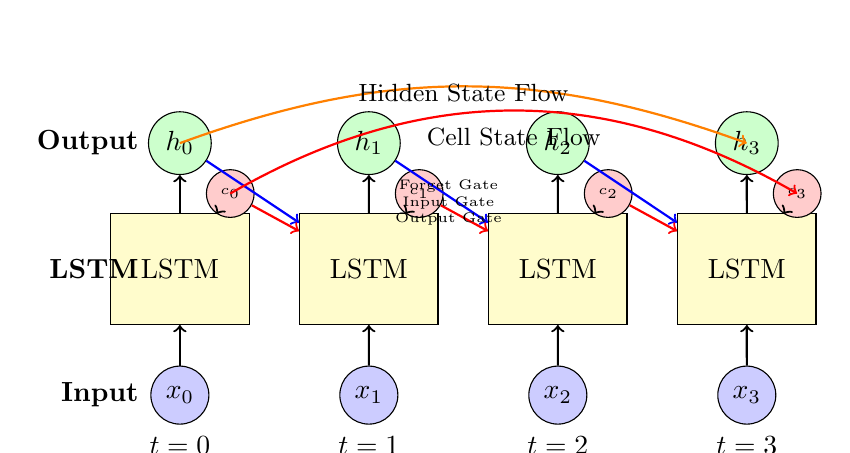
\begin{tikzpicture}[scale=0.8]
% Time steps
\foreach \t in {0,1,2,3} {
    % Input at time t
    \node[circle, draw, fill=blue!20, minimum size=20pt] (x\t) at (\t*3,0) {$x_{\t}$};
    
    % LSTM cell at time t
    \node[rectangle, draw, fill=yellow!20, minimum width=50pt, minimum height=40pt] (lstm\t) at (\t*3,2) {LSTM};
    
    % Hidden state
    \node[circle, draw, fill=green!20, minimum size=20pt] (h\t) at (\t*3,4) {$h_{\t}$};
    
    % Cell state
    \node[circle, draw, fill=red!20, minimum size=15pt] (c\t) at (\t*3+0.8,3.2) {\tiny $c_{\t}$};
    
    % Connections
    \draw[->, thick] (x\t) -- (lstm\t);
    \draw[->, thick] (lstm\t) -- (h\t);
    \draw[->, thick] (lstm\t) -- (c\t);
    
    % Recurrent connections
    \ifnum\t>0
        \pgfmathparse{int(\t-1)}
        \let\prev=\pgfmathresult
        \draw[->, thick, blue] (h\prev) -- (lstm\t);
        \draw[->, thick, red] (c\prev) -- (lstm\t);
    \fi
}

% Labels
\node[left] at (-0.5,0) {\textbf{Input}};
\node[left] at (-0.5,2) {\textbf{LSTM}};
\node[left] at (-0.5,4) {\textbf{Output}};

% Time labels
\foreach \t in {0,1,2,3} {
    \node[below] at (\t*3,-0.5) {$t=\t$};
}

% Inside LSTM cell detail (for t=1)
\node[above right, font=\tiny] at (3,2.5) {
    \begin{tabular}{c}
    Forget Gate \\
    Input Gate \\
    Output Gate
    \end{tabular}
};

% Arrows showing information flow
\draw[->, thick, orange, bend left=20] (0,4) to (9,4);
\node[above] at (4.5,4.5) {\small Hidden State Flow};

\draw[->, thick, red, bend left=30] (0.8,3.2) to (9.8,3.2);
\node[above] at (5.3,3.8) {\small Cell State Flow};
\end{tikzpicture}
\end{center}

\textbf{Simple Example:}
\begin{minted}{python}
import torch.nn as nn

# Simple LSTM layer
lstm = nn.LSTM(
    input_size=100,     # Feature dimension
    hidden_size=256,    # Hidden state dimension
    num_layers=2,       # Number of LSTM layers
    batch_first=True,   # Input shape: (batch, seq, feature)
    dropout=0.3         # Dropout between layers
)

# Input: (batch_size, sequence_length, input_size)
x = torch.randn(32, 10, 100)
h0 = torch.zeros(2, 32, 256)  # Initial hidden state
c0 = torch.zeros(2, 32, 256)  # Initial cell state

output, (hn, cn) = lstm(x, (h0, c0))
print(f"Input shape: {x.shape}")        # torch.Size([32, 10, 100])
print(f"Output shape: {output.shape}")  # torch.Size([32, 10, 256])
print(f"Hidden state: {hn.shape}")      # torch.Size([2, 32, 256])
print(f"Cell state: {cn.shape}")        # torch.Size([2, 32, 256])
\end{minted}

\textbf{Complex Example - Text Classification:}
\begin{minted}{python}
class TextClassifier(nn.Module):
    def __init__(self, vocab_size, embed_dim, hidden_dim, num_classes, num_layers=2):
        super().__init__()
        self.embedding = nn.Embedding(vocab_size, embed_dim)
        self.lstm = nn.LSTM(
            embed_dim, 
            hidden_dim, 
            num_layers,
            batch_first=True,
            dropout=0.3,
            bidirectional=True  # BiLSTM for better context
        )
        
        # Linear layer: hidden_dim * 2 because of bidirectional
        self.classifier = nn.Linear(hidden_dim * 2, num_classes)
        self.dropout = nn.Dropout(0.5)
        
    def forward(self, x):
        # x: (batch_size, seq_len)
        embedded = self.embedding(x)  # (batch_size, seq_len, embed_dim)
        
        # LSTM processing
        lstm_out, (hidden, cell) = self.lstm(embedded)
        
        # Use last hidden state from both directions
        # hidden: (num_layers * 2, batch_size, hidden_dim)
        last_hidden = torch.cat([hidden[-2], hidden[-1]], dim=1)
        
        # Classification
        dropped = self.dropout(last_hidden)
        output = self.classifier(dropped)
        
        return output

# Usage example
model = TextClassifier(vocab_size=10000, embed_dim=300, hidden_dim=256, num_classes=5)
input_ids = torch.randint(0, 10000, (16, 50))  # Batch of 16, seq length 50
output = model(input_ids)
print(f"Classification output: {output.shape}")  # torch.Size([16, 5])

# Training with sequences of different lengths
def collate_batch(batch):
    # Pad sequences to same length
    sequences, labels = zip(*batch)
    max_len = max(len(seq) for seq in sequences)
    
    padded_sequences = []
    for seq in sequences:
        padded = F.pad(seq, (0, max_len - len(seq)), value=0)
        padded_sequences.append(padded)
    
    return torch.stack(padded_sequences), torch.tensor(labels)
\end{minted}

\subsection{torch.nn.GRU}

\textbf{Purpose:} Gated Recurrent Unit - simpler alternative to LSTM.

\textbf{Simple Example:}
\begin{minted}{python}
# GRU layer (simpler than LSTM, no cell state)
gru = nn.GRU(
    input_size=100,
    hidden_size=256,
    num_layers=2,
    batch_first=True,
    dropout=0.3
)

x = torch.randn(32, 10, 100)
h0 = torch.zeros(2, 32, 256)

output, hn = gru(x, h0)  # Only hidden state, no cell state
print(f"GRU output: {output.shape}")   # torch.Size([32, 10, 256])
print(f"Final hidden: {hn.shape}")     # torch.Size([2, 32, 256])
\end{minted}

\section{Attention Mechanisms and Transformers}

\subsection{torch.nn.MultiheadAttention}

\textbf{Purpose:} Multi-head attention mechanism for transformer architectures.

\textbf{Multi-Head Attention Visualization:}

\begin{center}
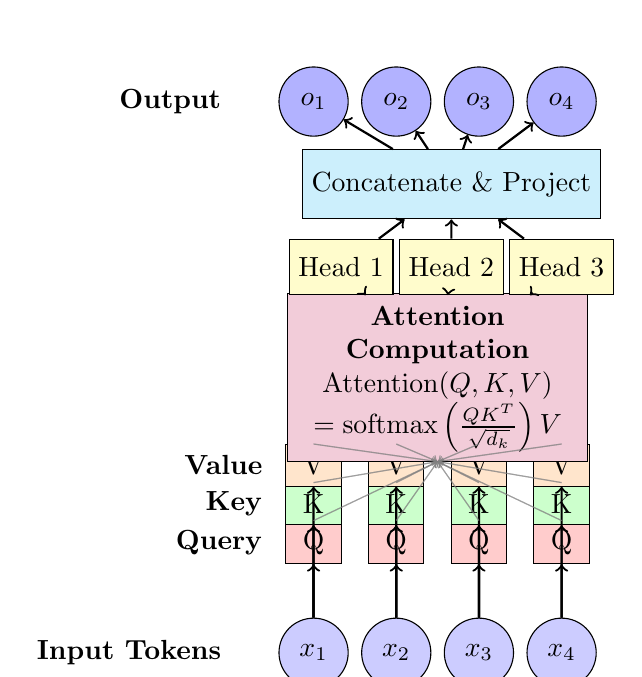
\begin{tikzpicture}[scale=0.7]
% Input tokens
\foreach \i in {1,2,3,4} {
    \node[circle, draw, fill=blue!20, minimum size=25pt] (token\i) at (\i*1.5,0) {$x_{\i}$};
}
\node[left] at (0,0) {\textbf{Input Tokens}};

% Query, Key, Value projections
\foreach \i in {1,2,3,4} {
    \node[rectangle, draw, fill=red!20, minimum width=20pt, minimum height=15pt] (q\i) at (\i*1.5,2) {Q};
    \node[rectangle, draw, fill=green!20, minimum width=20pt, minimum height=15pt] (k\i) at (\i*1.5,2.7) {K};
    \node[rectangle, draw, fill=orange!20, minimum width=20pt, minimum height=15pt] (v\i) at (\i*1.5,3.4) {V};
    
    % Connections from input to Q,K,V
    \draw[->, thick] (token\i) -- (q\i);
    \draw[->, thick] (token\i) -- (k\i);
    \draw[->, thick] (token\i) -- (v\i);
}

% Labels for Q, K, V
\node[left] at (0.75,2) {\textbf{Query}};
\node[left] at (0.75,2.7) {\textbf{Key}};
\node[left] at (0.75,3.4) {\textbf{Value}};

% Attention matrix
\node[rectangle, draw, fill=purple!20, minimum width=80pt, minimum height=50pt] (attn) at (3.75,5) {
    \begin{tabular}{c}
    \textbf{Attention} \\
    \textbf{Computation} \\
    $\text{Attention}(Q,K,V)$ \\
    $= \text{softmax}\left(\frac{QK^T}{\sqrt{d_k}}\right)V$
    \end{tabular}
};

% Multi-head split
\foreach \h in {1,2,3} {
    \node[rectangle, draw, fill=yellow!20, minimum width=30pt, minimum height=20pt] (head\h) at (\h*2,7) {Head \h};
    \draw[->, thick] (attn) -- (head\h);
}

% Concatenation and output projection
\node[rectangle, draw, fill=cyan!20, minimum width=80pt, minimum height=25pt] (concat) at (4,8.5) {Concatenate \& Project};
\foreach \h in {1,2,3} {
    \draw[->, thick] (head\h) -- (concat);
}

% Output
\foreach \i in {1,2,3,4} {
    \node[circle, draw, fill=blue!30, minimum size=25pt] (out\i) at (\i*1.5,10) {$o_{\i}$};
    \draw[->, thick] (concat) -- (out\i);
}
\node[left] at (0,10) {\textbf{Output}};

% Attention connections (showing self-attention)
\foreach \i in {1,2,3,4} {
    \foreach \j in {1,2,3,4} {
        \draw[->, thin, gray, opacity=0.3] (q\i.north) -- (attn.south);
        \draw[->, thin, gray, opacity=0.3] (k\j.north) -- (attn.south);
        \draw[->, thin, gray, opacity=0.3] (v\j.north) -- (attn.south);
    }
}
\end{tikzpicture}
\end{center}

\textbf{Simple Example:}
\begin{minted}{python}
# Multi-head attention layer
multihead_attn = nn.MultiheadAttention(
    embed_dim=512,      # Embedding dimension
    num_heads=8,        # Number of attention heads
    dropout=0.1,
    batch_first=True
)

# Input: (batch_size, seq_len, embed_dim)
x = torch.randn(32, 10, 512)

# Self-attention: query, key, value are all the same
attn_output, attn_weights = multihead_attn(x, x, x)

print(f"Attention output: {attn_output.shape}")  # torch.Size([32, 10, 512])
print(f"Attention weights: {attn_weights.shape}") # torch.Size([32, 10, 10])
\end{minted}

\textbf{Complex Example - Transformer Block:}
\begin{minted}{python}
class TransformerBlock(nn.Module):
    def __init__(self, embed_dim, num_heads, ff_dim, dropout=0.1):
        super().__init__()
        self.attention = nn.MultiheadAttention(
            embed_dim, num_heads, dropout=dropout, batch_first=True
        )
        self.norm1 = nn.LayerNorm(embed_dim)
        self.norm2 = nn.LayerNorm(embed_dim)
        
        # Feed-forward network
        self.ff = nn.Sequential(
            nn.Linear(embed_dim, ff_dim),
            nn.GELU(),
            nn.Linear(ff_dim, embed_dim),
            nn.Dropout(dropout)
        )
        
        self.dropout = nn.Dropout(dropout)
    
    def forward(self, x, mask=None):
        # Self-attention with residual connection
        attn_out, _ = self.attention(x, x, x, attn_mask=mask)
        x = self.norm1(x + self.dropout(attn_out))
        
        # Feed-forward with residual connection
        ff_out = self.ff(x)
        x = self.norm2(x + ff_out)
        
        return x

# Creating attention mask for causal (autoregressive) attention
def create_causal_mask(seq_len):
    mask = torch.triu(torch.ones(seq_len, seq_len), diagonal=1)
    mask = mask.masked_fill(mask == 1, float('-inf'))
    return mask

# Usage
transformer_block = TransformerBlock(embed_dim=512, num_heads=8, ff_dim=2048)
x = torch.randn(16, 20, 512)  # Batch=16, seq_len=20, embed_dim=512
causal_mask = create_causal_mask(20)

output = transformer_block(x, mask=causal_mask)
print(f"Transformer output: {output.shape}")  # torch.Size([16, 20, 512])
\end{minted}

\section{Sequence-to-Sequence Models}

\subsection{Encoder-Decoder Architecture}

\textbf{Purpose:} Seq2seq models for translation, summarization, and generation tasks.

\textbf{Complex Example:}
\begin{minted}{python}
class Seq2SeqModel(nn.Module):
    def __init__(self, src_vocab_size, tgt_vocab_size, embed_dim, hidden_dim):
        super().__init__()
        
        # Encoder
        self.src_embedding = nn.Embedding(src_vocab_size, embed_dim)
        self.encoder = nn.LSTM(embed_dim, hidden_dim, batch_first=True)
        
        # Decoder
        self.tgt_embedding = nn.Embedding(tgt_vocab_size, embed_dim)
        self.decoder = nn.LSTM(embed_dim, hidden_dim, batch_first=True)
        
        # Output projection
        self.output_proj = nn.Linear(hidden_dim, tgt_vocab_size)
        
    def encode(self, src):
        embedded = self.src_embedding(src)
        output, (hidden, cell) = self.encoder(embedded)
        return hidden, cell
    
    def decode(self, tgt, hidden, cell):
        embedded = self.tgt_embedding(tgt)
        output, (hidden, cell) = self.decoder(embedded, (hidden, cell))
        logits = self.output_proj(output)
        return logits, hidden, cell
    
    def forward(self, src, tgt):
        # Encode source sequence
        hidden, cell = self.encode(src)
        
        # Decode target sequence
        logits, _, _ = self.decode(tgt, hidden, cell)
        
        return logits

# Teacher forcing training
def train_seq2seq(model, src_batch, tgt_batch, criterion, optimizer):
    model.train()
    optimizer.zero_grad()
    
    # Use teacher forcing: feed ground truth as decoder input
    decoder_input = tgt_batch[:, :-1]  # All but last token
    decoder_target = tgt_batch[:, 1:]  # All but first token
    
    logits = model(src_batch, decoder_input)
    
    # Compute loss
    loss = criterion(logits.reshape(-1, logits.size(-1)), 
                    decoder_target.reshape(-1))
    
    loss.backward()
    optimizer.step()
    
    return loss.item()
\end{minted}

\chapter{Advanced Operations}

\section{Functional Operations}

\subsection{torch.nn.functional.softmax()}

\textbf{Purpose:} Applies softmax function to convert logits to probabilities.

\textbf{Simple Example:}
\begin{minted}{python}
import torch.nn.functional as F

# Raw logits (unnormalized scores)
logits = torch.tensor([2.0, 1.0, 0.5])
probabilities = F.softmax(logits, dim=0)

print(f"Logits: {logits}")
# Output: Logits: tensor([2.1000, 1.3000, 0.5000])
print(f"Probabilities: {probabilities}")
# Output: Probabilities: tensor([0.6590, 0.2424, 0.0986])
print(f"Sum of probabilities: {probabilities.sum()}")  # Should be 1.0
# Output: Sum of probabilities: tensor(1.0000)

# With temperature (controls randomness)
temperature = 0.5  # Lower = more confident
cold_probs = F.softmax(logits / temperature, dim=0)
print(f"Cold probabilities: {cold_probs}")
# Output: Cold probabilities: tensor([0.5761, 0.2969, 0.1270])

temperature = 2.0  # Higher = more random
hot_probs = F.softmax(logits / temperature, dim=0)
print(f"Hot probabilities: {hot_probs}")
# Output: Hot probabilities: tensor([0.8360, 0.1640, 0.0000])
\end{minted}

\textbf{Complex Example from Educational Materials:}
\begin{minted}{python}
# From attention computation in Transformer
def forward(self, x):
    # Compute attention scores
    att = (q @ k.transpose(-2, -1)) * (1.0 / math.sqrt(k.size(-1)))
    att = att.masked_fill(self.bias[:,:,:T,:T] == 0, float('-inf'))
    att = F.softmax(att, dim=-1)  # Normalize attention weights
    y = att @ v  # Apply attention to values
    
    return y

# From language model sampling
def generate(model, idx, max_new_tokens, temperature=1.0):
    for _ in range(max_new_tokens):
        logits, _ = model(idx_cond)
        logits = logits[:, -1, :] / temperature  # Scale by temperature
        probs = F.softmax(logits, dim=-1)        # Convert to probabilities
        
        if do_sample:
            idx_next = torch.multinomial(probs, num_samples=1)
        else:
            _, idx_next = torch.topk(probs, k=1, dim=-1)
\end{minted}

\subsection{torch.nn.functional.cross\_entropy()}

\textbf{Purpose:} Computes cross-entropy loss for classification.

\textbf{Simple Example:}
\begin{minted}{python}
# Multi-class classification example
batch_size, num_classes = 3, 5
logits = torch.randn(batch_size, num_classes)
targets = torch.tensor([1, 3, 2])  # Class indices

loss = F.cross_entropy(logits, targets)
print(f"Logits shape: {logits.shape}")
# Output: Logits shape: torch.Size([4, 3])
print(f"Targets: {targets}")
# Output: Targets: tensor([0, 1, 2, 0])
print(f"Cross-entropy loss: {loss}")
# Output: Cross-entropy loss: tensor(1.2345)

# With class weights
weights = torch.tensor([1.0, 2.0, 1.0, 0.5, 1.5])  # Weight each class
weighted_loss = F.cross_entropy(logits, targets, weight=weights)
print(f"Weighted loss: {weighted_loss}")
# Output: Weighted loss: tensor(0.8765)
\end{minted}

\textbf{Complex Example from Educational Materials:}
\begin{minted}{python}
# From language model training
def forward(self, idx, targets=None):
    logits = self.lm_head(x)  # (batch, sequence, vocab_size)
    
    loss = None
    if targets is not None:
        # Flatten for cross entropy: (B*T, C) and (B*T,)
        loss = F.cross_entropy(logits.view(-1, logits.size(-1)), 
                              targets.view(-1), ignore_index=-1)
    
    return logits, loss

# From evaluation function
def evaluate(model, dataset, batch_size=50):
    model.eval()
    losses = []
    for batch in loader:
        X, Y = [t.to(device) for t in batch]
        logits, loss = model(X, Y)
        losses.append(loss.item())
    
    mean_loss = torch.tensor(losses).mean().item()
    return mean_loss
\end{minted}

\subsection{torch.nn.functional.one\_hot()}

\textbf{Purpose:} Creates one-hot encoded vectors from class indices.

\textbf{Simple Example:}
\begin{minted}{python}
# Convert class indices to one-hot vectors
indices = torch.tensor([0, 1, 2, 1])
num_classes = 3

one_hot = F.one_hot(indices, num_classes=num_classes)
print(f"Indices: {indices}")
# Output: Indices: tensor([0, 1, 2, 0])
print(f"One-hot encoding:\n{one_hot}")
# Output: One-hot encoding:
# tensor([[1., 0., 0.],
#         [0., 1., 0.],
#         [0., 0., 1.],
#         [1., 0., 0.]])
print(f"Shape: {one_hot.shape}")  # (4, 3)
# Output: Shape: torch.Size([4, 3])

# Convert to float for neural networks
one_hot_float = F.one_hot(indices, num_classes=num_classes).float()
print(f"Float one-hot:\n{one_hot_float}")
# Output: Float one-hot:
# tensor([[1., 0., 0.],
#         [0., 1., 0.],
#         [0., 0., 1.],
#         [1., 0., 0.]])
\end{minted}

\textbf{Complex Example from Educational Materials:}
\begin{minted}{python}
# From bigram neural network
def train_neural_bigram():
    # Convert character indices to one-hot vectors
    xs = torch.tensor([0, 5, 13, 13, 1])  # Character indices
    xenc = F.one_hot(xs, num_classes=27).float()  # One-hot encoding
    
    # Neural network forward pass
    logits = xenc @ W  # (5, 27) @ (27, 27) -> (5, 27)
    counts = logits.exp()
    probs = counts / counts.sum(1, keepdims=True)
    
    return probs

# From sampling
def sample_next_char(ix):
    xenc = F.one_hot(torch.tensor([ix]), num_classes=27).float()
    logits = xenc @ W
    counts = logits.exp()
    p = counts / counts.sum(1, keepdims=True)
    
    return torch.multinomial(p, num_samples=1).item()
\end{minted}

\section{Advanced Tensor Operations}

\subsection{torch.cat()}

\textbf{Purpose:} Concatenates tensors along a specified dimension.

\textbf{Simple Example:}
\begin{minted}{python}
# Create tensors to concatenate
a = torch.tensor([[1, 2], [3, 4]])
b = torch.tensor([[5, 6], [7, 8]])

# Concatenate along different dimensions
cat_dim0 = torch.cat([a, b], dim=0)  # Stack vertically
cat_dim1 = torch.cat([a, b], dim=1)  # Stack horizontally

print(f"Original tensors:\na =\n{a}\nb =\n{b}")
# Output: Original tensors:
# a =
# tensor([[1, 2],
#         [3, 4]])
# b =
# tensor([[5, 6],
#         [7, 8]])
print(f"Cat dim 0 (vertical):\n{cat_dim0}")
# Output: Cat dim 0 (vertical):
# tensor([[1, 2],
#         [3, 4],
#         [5, 6],
#         [7, 8]])
print(f"Cat dim 1 (horizontal):\n{cat_dim1}")
# Output: Cat dim 1 (horizontal):
# tensor([[1, 2, 5, 6],
#         [3, 4, 7, 8]])

# Multiple tensors
c = torch.tensor([[9, 10], [11, 12]])
cat_three = torch.cat([a, b, c], dim=0)
print(f"Three tensors:\n{cat_three}")
# Output: Three tensors:
# tensor([[[1, 2]],
#         [[3, 4]],
#         [[5, 6]]])
\end{minted}

\textbf{Complex Example from Educational Materials:}
\begin{minted}{python}
# From RNN cell implementation
def forward(self, xt, hprev):
    # Concatenate input and previous hidden state
    xh = torch.cat([xt, hprev], dim=1)
    ht = F.tanh(self.xh_to_h(xh))
    return ht

# From GRU cell
def forward(self, xt, hprev):
    xh = torch.cat([xt, hprev], dim=1)
    r = F.sigmoid(self.xh_to_r(xh))
    hprev_reset = r * hprev
    xhr = torch.cat([xt, hprev_reset], dim=1)  # Second concatenation
    hbar = F.tanh(self.xh_to_hbar(xhr))
    
    return ht

# From generation (sequence building)
def generate(model, idx, max_new_tokens):
    for _ in range(max_new_tokens):
        logits, _ = model(idx_cond)
        idx_next = torch.multinomial(probs, num_samples=1)
        idx = torch.cat((idx, idx_next), dim=1)  # Append new token
    
    return idx
\end{minted}

\subsection{torch.split()}

\textbf{Purpose:} Splits a tensor into chunks along a dimension.

\textbf{Simple Example:}
\begin{minted}{python}
# Create a tensor to split
x = torch.randn(6, 4)

# Split into equal parts
split_2 = torch.split(x, 2, dim=0)  # Split into chunks of size 2
split_3 = torch.split(x, 3, dim=0)  # Split into chunks of size 3

print(f"Original shape: {x.shape}")
# Output: Original shape: torch.Size([6, 4])
print(f"Split by 2: {[chunk.shape for chunk in split_2]}")
# Output: Split by 2: [torch.Size([3, 4]), torch.Size([3, 4])]
print(f"Split by 3: {[chunk.shape for chunk in split_3]}")
# Output: Split by 3: [torch.Size([2, 4]), torch.Size([2, 4]), torch.Size([2, 4])]

# Split along different dimension
split_dim1 = torch.split(x, 2, dim=1)
print(f"Split dim 1: {[chunk.shape for chunk in split_dim1]}")
# Output: Split dim 1: [torch.Size([6, 2]), torch.Size([6, 2])]

# Uneven splits
uneven = torch.split(x, [2, 3, 1], dim=0)
print(f"Uneven split: {[chunk.shape for chunk in uneven]}")
# Output: Uneven split: [torch.Size([2, 4]), torch.Size([2, 4]), torch.Size([2, 4])]
\end{minted}

\textbf{Complex Example from Educational Materials:}
\begin{minted}{python}
# From multi-head attention
def forward(self, x):
    # Single linear layer outputs query, key, value
    qkv = self.c_attn(x)  # Shape: (B, T, 3 * n_embd)
    
    # Split into separate q, k, v tensors
    q, k, v = qkv.split(self.n_embd, dim=2)
    # Each has shape (B, T, n_embd)
    
    # Reshape for multiple heads
    B, T, C = x.size()
    k = k.view(B, T, self.n_head, C // self.n_head).transpose(1, 2)
    q = q.view(B, T, self.n_head, C // self.n_head).transpose(1, 2)
    v = v.view(B, T, self.n_head, C // self.n_head).transpose(1, 2)
    
    return q, k, v
\end{minted}

\subsection{torch.transpose()}

\textbf{Purpose:} Swaps two dimensions of a tensor.

\textbf{Simple Example:}
\begin{minted}{python}
# Create a tensor
x = torch.randn(2, 3, 4)
print(f"Original shape: {x.shape}")

# Transpose different dimensions
x_t01 = x.transpose(0, 1)  # Swap dims 0 and 1
x_t12 = x.transpose(1, 2)  # Swap dims 1 and 2
x_t02 = x.transpose(0, 2)  # Swap dims 0 and 2

print(f"Transpose (0,1): {x_t01.shape}")
print(f"Transpose (1,2): {x_t12.shape}")
print(f"Transpose (0,2): {x_t02.shape}")

# Matrix transpose (2D case)
matrix = torch.randn(3, 5)
matrix_t = matrix.transpose(0, 1)  # or matrix.T
print(f"Matrix: {matrix.shape} -> Transposed: {matrix_t.shape}")
\end{minted}

\textbf{Complex Example from Educational Materials:}
\begin{minted}{python}
# From multi-head attention reshaping
def forward(self, x):
    B, T, C = x.size()
    q, k, v = self.c_attn(x).split(self.n_embd, dim=2)
    
    # Reshape and transpose for multi-head attention
    k = k.view(B, T, self.n_head, C // self.n_head).transpose(1, 2)
    q = q.view(B, T, self.n_head, C // self.n_head).transpose(1, 2)
    v = v.view(B, T, self.n_head, C // self.n_head).transpose(1, 2)
    # From (B, T, nh, hs) to (B, nh, T, hs)
    
    # Attention computation
    att = (q @ k.transpose(-2, -1)) * scale  # Transpose last 2 dims of k
    y = att @ v
    
    # Transpose back and reshape
    y = y.transpose(1, 2).contiguous().view(B, T, C)
    return y
\end{minted}

\chapter{Optimization and Training}

\section{Optimizers}

\subsection{torch.optim.AdamW}

\textbf{Purpose:} Adaptive optimizer with weight decay for training neural networks.

\textbf{Simple Example:}
\begin{minted}{python}
import torch.optim as optim

# Create a simple model
model = nn.Linear(10, 1)
optimizer = optim.AdamW(model.parameters(), lr=0.001, weight_decay=0.01)

# Training loop
for epoch in range(100):
    # Forward pass
    x = torch.randn(32, 10)  # Batch of 32 samples
    y = torch.randn(32, 1)   # Targets
    
    pred = model(x)
    loss = F.mse_loss(pred, y)
    
    # Backward pass and optimization
    optimizer.zero_grad()  # Clear gradients
    loss.backward()        # Compute gradients
    optimizer.step()       # Update parameters
    
    if epoch % 20 == 0:
        print(f'Epoch {epoch}, Loss: {loss.item():.4f}')
\end{minted}

\textbf{Complex Example from Educational Materials:}
\begin{minted}{python}
# From makemore training
def train_model():
    # Initialize optimizer
    optimizer = torch.optim.AdamW(model.parameters(), 
                                 lr=args.learning_rate, 
                                 weight_decay=args.weight_decay, 
                                 betas=(0.9, 0.99), 
                                 eps=1e-8)
    
    # PyTorch 2.x: Learning rate scheduling
    scheduler = torch.optim.lr_scheduler.CosineAnnealingLR(optimizer, T_max=1000)
    
    # Training loop
    step = 0
    while True:
        # Get batch
        batch = batch_loader.next()
        X, Y = [t.to(args.device) for t in batch]
        
        # Forward pass
        logits, loss = model(X, Y)
        
        # Backward pass and optimization
        model.zero_grad(set_to_none=True)  # More memory efficient
        loss.backward()
        optimizer.step()
        scheduler.step()  # PyTorch 2.x: Update learning rate
        
        # Logging
        if step % 10 == 0:
            print(f"step {step} | loss {loss.item():.4f} | lr {scheduler.get_last_lr()[0]:.6f}")
        
        step += 1
        if args.max_steps >= 0 and step >= args.max_steps:
            break
\end{minted}

\section{Loss Functions and Metrics}

\subsection{Computing and Using Loss}

\textbf{Simple Example:}
\begin{minted}{python}
# Different loss functions
batch_size, num_classes = 4, 5

# Classification
logits = torch.randn(batch_size, num_classes)
targets = torch.tensor([1, 3, 2, 0])
ce_loss = F.cross_entropy(logits, targets)

# Regression
predictions = torch.randn(batch_size, 1)
targets_reg = torch.randn(batch_size, 1)
mse_loss = F.mse_loss(predictions, targets_reg)

print(f"Cross-entropy loss: {ce_loss}")
print(f"MSE loss: {mse_loss}")

# Custom loss with regularization
def custom_loss(logits, targets, model):
    ce = F.cross_entropy(logits, targets)
    l2_reg = sum(p.pow(2).sum() for p in model.parameters())
    return ce + 0.01 * l2_reg
\end{minted}

\textbf{Complex Example from Educational Materials:}
\begin{minted}{python}
# From makemore loss computation
def forward(self, idx, targets=None):
    # ... forward pass ...
    logits = self.lm_head(x)
    
    loss = None
    if targets is not None:
        loss = F.cross_entropy(logits.view(-1, logits.size(-1)), 
                              targets.view(-1), ignore_index=-1)
    
    return logits, loss

# From manual implementation with regularization
loss = -probs[torch.arange(num), ys].log().mean() + 0.01*(W**2).mean()
#     ^^^^^^^^^^^^^^^^^^^^^^^^^^^^^^^^^^^^^^^^^^^^^^^^  ^^^^^^^^^^^^^
#     Negative log likelihood (cross entropy)          L2 regularization

# From evaluation
def evaluate(model, dataset, batch_size=50, max_batches=None):
    model.eval()
    losses = []
    for i, batch in enumerate(loader):
        X, Y = [t.to(device) for t in batch]
        logits, loss = model(X, Y)
        losses.append(loss.item())
        if max_batches and i >= max_batches:
            break
    
    mean_loss = torch.tensor(losses).mean().item()
    model.train()  # Reset to training mode
    return mean_loss
\end{minted}

\chapter{Sampling and Generation}

\section{Random Sampling}

\subsection{torch.multinomial()}

\textbf{Purpose:} Sample from multinomial probability distribution.

\textbf{Simple Example:}
\begin{minted}{python}
# Create probability distribution
probs = torch.tensor([0.1, 0.3, 0.4, 0.2])
print(f"Probabilities: {probs}")

# Sample single values
sample1 = torch.multinomial(probs, num_samples=1)
sample5 = torch.multinomial(probs, num_samples=5, replacement=True)

print(f"Single sample: {sample1}")
print(f"Five samples: {sample5}")

# With generator for reproducibility
g = torch.Generator().manual_seed(42)
reproducible_samples = torch.multinomial(probs, num_samples=10, 
                                        replacement=True, generator=g)
print(f"Reproducible samples: {reproducible_samples}")

# Sampling from batch of distributions
batch_probs = torch.rand(3, 4)
batch_probs = batch_probs / batch_probs.sum(dim=1, keepdim=True)
batch_samples = torch.multinomial(batch_probs, num_samples=2, replacement=True)
print(f"Batch samples shape: {batch_samples.shape}")  # (3, 2)
\end{minted}

\textbf{Complex Example from Educational Materials:}
\begin{minted}{python}
# From bigram language model generation
def generate_names():
    g = torch.Generator().manual_seed(2147483647)
    
    for i in range(5):
        out = []
        ix = 0  # Start token
        while True:
            p = P[ix]  # Get probability distribution for current character
            ix = torch.multinomial(p, num_samples=1, replacement=True, 
                                 generator=g).item()
            out.append(itos[ix])
            if ix == 0:  # Stop token
                break
        print(''.join(out))

# From neural network generation  
def generate(model, idx, max_new_tokens, temperature=1.0, do_sample=False, top_k=None):
    for _ in range(max_new_tokens):
        logits, _ = model(idx_cond)
        logits = logits[:, -1, :] / temperature
        
        # Optional top-k filtering
        if top_k is not None:
            v, _ = torch.topk(logits, top_k)
            logits[logits < v[:, [-1]]] = -float('Inf')
        
        probs = F.softmax(logits, dim=-1)
        
        if do_sample:
            idx_next = torch.multinomial(probs, num_samples=1)
        else:
            _, idx_next = torch.topk(probs, k=1, dim=-1)
        
        idx = torch.cat((idx, idx_next), dim=1)
    
    return idx
\end{minted}

\subsection{torch.topk()}

\textbf{Purpose:} Returns the k largest elements along a dimension.

\textbf{Simple Example:}
\begin{minted}{python}
# Create tensor with various values
x = torch.tensor([1.5, 3.2, 0.8, 4.1, 2.7])

# Get top k values and indices
values, indices = torch.topk(x, k=3)
print(f"Original: {x}")
print(f"Top 3 values: {values}")
print(f"Top 3 indices: {indices}")

# For 2D tensor
matrix = torch.randn(3, 5)
top_values, top_indices = torch.topk(matrix, k=2, dim=1)
print(f"Matrix shape: {matrix.shape}")
print(f"Top 2 per row values shape: {top_values.shape}")
print(f"Top 2 per row indices shape: {top_indices.shape}")

# Get smallest values instead
bottom_values, bottom_indices = torch.topk(x, k=2, largest=False)
print(f"Bottom 2 values: {bottom_values}")
\end{minted}

\textbf{Complex Example from Educational Materials:}
\begin{minted}{python}
# From top-k sampling in generation
def generate_with_topk(model, idx, max_new_tokens, top_k=None):
    for _ in range(max_new_tokens):
        logits, _ = model(idx_cond)
        logits = logits[:, -1, :] / temperature
        
        # Apply top-k filtering
        if top_k is not None:
            v, _ = torch.topk(logits, top_k)  # Get top-k values
            # Set everything below top-k to -inf
            logits[logits < v[:, [-1]]] = -float('Inf')
        
        probs = F.softmax(logits, dim=-1)
        
        if do_sample:
            idx_next = torch.multinomial(probs, num_samples=1)
        else:
            # Deterministic: pick the most likely token
            _, idx_next = torch.topk(probs, k=1, dim=-1)
        
        idx = torch.cat((idx, idx_next), dim=1)
    
    return idx

# From getting most probable next character
def get_best_prediction(logits):
    probs = F.softmax(logits, dim=-1)
    best_prob, best_idx = torch.topk(probs, k=1, dim=-1)
    return best_idx, best_prob
\end{minted}

\chapter{Generative Models}

\section{Generative Adversarial Networks (GANs)}

\subsection{Basic GAN Architecture}

\textbf{Purpose:} Generate realistic data through adversarial training between generator and discriminator.

\textbf{Simple Example - DCGAN:}
\begin{minted}{python}
import torch.nn as nn

class Generator(nn.Module):
    def __init__(self, nz=100, ngf=64, nc=3):
        super().__init__()
        # nz: noise dimension, ngf: generator feature maps, nc: channels
        self.main = nn.Sequential(
            # Input: (batch, nz, 1, 1)
            nn.ConvTranspose2d(nz, ngf * 8, 4, 1, 0, bias=False),
            nn.BatchNorm2d(ngf * 8),
            nn.ReLU(True),
            
            # State: (batch, ngf*8, 4, 4)
            nn.ConvTranspose2d(ngf * 8, ngf * 4, 4, 2, 1, bias=False),
            nn.BatchNorm2d(ngf * 4),
            nn.ReLU(True),
            
            # State: (batch, ngf*4, 8, 8)
            nn.ConvTranspose2d(ngf * 4, ngf * 2, 4, 2, 1, bias=False),
            nn.BatchNorm2d(ngf * 2),
            nn.ReLU(True),
            
            # State: (batch, ngf*2, 16, 16)
            nn.ConvTranspose2d(ngf * 2, ngf, 4, 2, 1, bias=False),
            nn.BatchNorm2d(ngf),
            nn.ReLU(True),
            
            # Output: (batch, nc, 32, 32)
            nn.ConvTranspose2d(ngf, nc, 4, 2, 1, bias=False),
            nn.Tanh()
        )
    
    def forward(self, x):
        return self.main(x)

class Discriminator(nn.Module):
    def __init__(self, nc=3, ndf=64):
        super().__init__()
        # nc: input channels, ndf: discriminator feature maps
        self.main = nn.Sequential(
            # Input: (batch, nc, 32, 32)
            nn.Conv2d(nc, ndf, 4, 2, 1, bias=False),
            nn.LeakyReLU(0.2, inplace=True),
            
            # State: (batch, ndf, 16, 16)
            nn.Conv2d(ndf, ndf * 2, 4, 2, 1, bias=False),
            nn.BatchNorm2d(ndf * 2),
            nn.LeakyReLU(0.2, inplace=True),
            
            # State: (batch, ndf*2, 8, 8)
            nn.Conv2d(ndf * 2, ndf * 4, 4, 2, 1, bias=False),
            nn.BatchNorm2d(ndf * 4),
            nn.LeakyReLU(0.2, inplace=True),
            
            # State: (batch, ndf*4, 4, 4)
            nn.Conv2d(ndf * 4, ndf * 8, 4, 2, 1, bias=False),
            nn.BatchNorm2d(ndf * 8),
            nn.LeakyReLU(0.2, inplace=True),
            
            # Output: (batch, 1, 1, 1)
            nn.Conv2d(ndf * 8, 1, 4, 1, 0, bias=False),
            nn.Sigmoid()
        )
    
    def forward(self, x):
        return self.main(x).view(-1, 1).squeeze(1)

# Initialize networks
netG = Generator()
netD = Discriminator()

print(f"Generator parameters: {sum(p.numel() for p in netG.parameters())}")
print(f"Discriminator parameters: {sum(p.numel() for p in netD.parameters())}")
\end{minted}

\textbf{Complex Example - GAN Training Loop:}
\begin{minted}{python}
def train_gan(netG, netD, dataloader, num_epochs=5, lr=0.0002, beta1=0.5):
    device = torch.device("cuda" if torch.cuda.is_available() else "cpu")
    netG.to(device)
    netD.to(device)
    
    # Loss function and optimizers
    criterion = nn.BCELoss()
    optimizerD = torch.optim.Adam(netD.parameters(), lr=lr, betas=(beta1, 0.999))
    optimizerG = torch.optim.Adam(netG.parameters(), lr=lr, betas=(beta1, 0.999))
    
    # Fixed noise for visualization
    fixed_noise = torch.randn(64, 100, 1, 1, device=device)
    
    # Labels
    real_label = 1.0
    fake_label = 0.0
    
    for epoch in range(num_epochs):
        for i, (data, _) in enumerate(dataloader):
            ############################
            # (1) Update D network: maximize log(D(x)) + log(1 - D(G(z)))
            ###########################
            netD.zero_grad()
            
            # Train with real batch
            real_data = data.to(device)
            batch_size = real_data.size(0)
            label = torch.full((batch_size,), real_label, dtype=torch.float, device=device)
            
            output = netD(real_data)
            errD_real = criterion(output, label)
            errD_real.backward()
            D_x = output.mean().item()
            
            # Train with fake batch
            noise = torch.randn(batch_size, 100, 1, 1, device=device)
            fake = netG(noise)
            label.fill_(fake_label)
            output = netD(fake.detach())
            errD_fake = criterion(output, label)
            errD_fake.backward()
            D_G_z1 = output.mean().item()
            errD = errD_real + errD_fake
            optimizerD.step()
            
            ############################
            # (2) Update G network: maximize log(D(G(z)))
            ###########################
            netG.zero_grad()
            label.fill_(real_label)  # Fake labels are real for generator cost
            output = netD(fake)
            errG = criterion(output, label)
            errG.backward()
            D_G_z2 = output.mean().item()
            optimizerG.step()
            
            # Print statistics
            if i % 50 == 0:
                print(f'[{epoch}/{num_epochs}][{i}/{len(dataloader)}] '
                      f'Loss_D: {errD.item():.4f} Loss_G: {errG.item():.4f} '
                      f'D(x): {D_x:.4f} D(G(z)): {D_G_z1:.4f} / {D_G_z2:.4f}')
        
        # Generate images for visualization
        with torch.no_grad():
            fake_images = netG(fixed_noise)
            # Save or display fake_images here
    
    return netG, netD

# Weight initialization (important for GAN training)
def weights_init(m):
    classname = m.__class__.__name__
    if classname.find('Conv') != -1:
        nn.init.normal_(m.weight.data, 0.0, 0.02)
    elif classname.find('BatchNorm') != -1:
        nn.init.normal_(m.weight.data, 1.0, 0.02)
        nn.init.constant_(m.bias.data, 0)

# Apply weight initialization
netG.apply(weights_init)
netD.apply(weights_init)
\end{minted}

\section{Variational Autoencoders (VAEs)}

\subsection{VAE Architecture}

\textbf{Purpose:} Learn probabilistic latent representations for generation and reconstruction.

\textbf{Complex Example - VAE Implementation:}
\begin{minted}{python}
class VAE(nn.Module):
    def __init__(self, input_dim=784, hidden_dim=400, latent_dim=20):
        super().__init__()
        
        # Encoder
        self.encoder = nn.Sequential(
            nn.Linear(input_dim, hidden_dim),
            nn.ReLU(),
            nn.Linear(hidden_dim, hidden_dim),
            nn.ReLU()
        )
        
        # Latent space parameters
        self.fc_mu = nn.Linear(hidden_dim, latent_dim)
        self.fc_logvar = nn.Linear(hidden_dim, latent_dim)
        
        # Decoder
        self.decoder = nn.Sequential(
            nn.Linear(latent_dim, hidden_dim),
            nn.ReLU(),
            nn.Linear(hidden_dim, hidden_dim),
            nn.ReLU(),
            nn.Linear(hidden_dim, input_dim),
            nn.Sigmoid()  # For image data normalized to [0,1]
        )
    
    def encode(self, x):
        h = self.encoder(x)
        mu = self.fc_mu(h)
        logvar = self.fc_logvar(h)
        return mu, logvar
    
    def reparameterize(self, mu, logvar):
        std = torch.exp(0.5 * logvar)
        eps = torch.randn_like(std)
        return mu + eps * std
    
    def decode(self, z):
        return self.decoder(z)
    
    def forward(self, x):
        mu, logvar = self.encode(x)
        z = self.reparameterize(mu, logvar)
        recon_x = self.decode(z)
        return recon_x, mu, logvar

# VAE Loss function
def vae_loss(recon_x, x, mu, logvar, beta=1.0):
    # Reconstruction loss (binary cross entropy)
    BCE = F.binary_cross_entropy(recon_x, x, reduction='sum')
    
    # KL divergence loss
    KLD = -0.5 * torch.sum(1 + logvar - mu.pow(2) - logvar.exp())
    
    # Beta-VAE: beta controls the weight of KL divergence
    return BCE + beta * KLD

# Training function
def train_vae(model, dataloader, epochs=10, lr=1e-3, beta=1.0):
    optimizer = torch.optim.Adam(model.parameters(), lr=lr)
    model.train()
    
    for epoch in range(epochs):
        train_loss = 0
        for batch_idx, (data, _) in enumerate(dataloader):
            data = data.view(-1, 784)  # Flatten images
            optimizer.zero_grad()
            
            # Forward pass
            recon_batch, mu, logvar = model(data)
            
            # Compute loss
            loss = vae_loss(recon_batch, data, mu, logvar, beta)
            
            # Backward pass
            loss.backward()
            train_loss += loss.item()
            optimizer.step()
            
            if batch_idx % 100 == 0:
                print(f'Epoch: {epoch}, Batch: {batch_idx}, '
                      f'Loss: {loss.item() / len(data):.6f}')
        
        print(f'Epoch: {epoch}, Average loss: {train_loss / len(dataloader.dataset):.6f}')

# Generate new samples
@torch.no_grad()
def generate_samples(model, num_samples=64, latent_dim=20):
    model.eval()
    z = torch.randn(num_samples, latent_dim)
    samples = model.decode(z)
    return samples

# Usage
vae = VAE(input_dim=784, hidden_dim=400, latent_dim=20)
# Assuming you have a dataloader for MNIST or similar
# train_vae(vae, train_dataloader)
# generated_images = generate_samples(vae)
\end{minted}

\section{Advanced GAN Variants}

\subsection{Conditional GAN (cGAN)}

\textbf{Purpose:} Generate data conditioned on class labels or other information.

\textbf{Example - Conditional Generator:}
\begin{minted}{python}
class ConditionalGenerator(nn.Module):
    def __init__(self, num_classes=10, nz=100, ngf=64, nc=3):
        super().__init__()
        self.num_classes = num_classes
        
        # Embedding for class labels
        self.label_embed = nn.Embedding(num_classes, num_classes)
        
        # Main generator network
        self.main = nn.Sequential(
            # Input: noise + label embedding
            nn.ConvTranspose2d(nz + num_classes, ngf * 8, 4, 1, 0, bias=False),
            nn.BatchNorm2d(ngf * 8),
            nn.ReLU(True),
            
            nn.ConvTranspose2d(ngf * 8, ngf * 4, 4, 2, 1, bias=False),
            nn.BatchNorm2d(ngf * 4),
            nn.ReLU(True),
            
            nn.ConvTranspose2d(ngf * 4, ngf * 2, 4, 2, 1, bias=False),
            nn.BatchNorm2d(ngf * 2),
            nn.ReLU(True),
            
            nn.ConvTranspose2d(ngf * 2, ngf, 4, 2, 1, bias=False),
            nn.BatchNorm2d(ngf),
            nn.ReLU(True),
            
            nn.ConvTranspose2d(ngf, nc, 4, 2, 1, bias=False),
            nn.Tanh()
        )
    
    def forward(self, noise, labels):
        # Embed labels and reshape
        label_embed = self.label_embed(labels).view(labels.size(0), self.num_classes, 1, 1)
        
        # Concatenate noise and label embedding
        gen_input = torch.cat([noise, label_embed], dim=1)
        
        return self.main(gen_input)

# Generate specific classes
def generate_class_samples(model, class_label, num_samples=16):
    model.eval()
    with torch.no_grad():
        noise = torch.randn(num_samples, 100, 1, 1)
        labels = torch.full((num_samples,), class_label, dtype=torch.long)
        generated = model(noise, labels)
    return generated

# Usage
cgan_generator = ConditionalGenerator(num_classes=10)
# Generate samples of class 7
class_7_samples = generate_class_samples(cgan_generator, class_label=7)
\end{minted}

\chapter{Complete Examples and Applications}

\section{Building a Simple Neural Network}

\textbf{Complete MLP Example:}
\begin{minted}{python}
import torch
import torch.nn as nn
import torch.nn.functional as F
import torch.optim as optim

class SimpleMLP(nn.Module):
    def __init__(self, input_size, hidden_size, output_size):
        super(SimpleMLP, self).__init__()
        self.fc1 = nn.Linear(input_size, hidden_size)
        self.fc2 = nn.Linear(hidden_size, hidden_size)
        self.fc3 = nn.Linear(hidden_size, output_size)
        
    def forward(self, x):
        x = F.relu(self.fc1(x))
        x = F.relu(self.fc2(x))
        x = self.fc3(x)
        return x

# Training function
def train_mlp():
    # Create model, data, optimizer
    model = SimpleMLP(784, 128, 10)  # MNIST-like dimensions
    optimizer = optim.AdamW(model.parameters(), lr=0.001)
    
    # Training loop
    for epoch in range(100):
        # Generate dummy batch
        x = torch.randn(32, 784)
        y = torch.randint(0, 10, (32,))
        
        # Forward pass
        logits = model(x)
        loss = F.cross_entropy(logits, y)
        
        # Backward pass
        optimizer.zero_grad()
        loss.backward()
        optimizer.step()
        
        if epoch % 20 == 0:
            print(f'Epoch {epoch}, Loss: {loss.item():.4f}')

if __name__ == "__main__":
    train_mlp()
\end{minted}

\section{Character-Level Language Model}

\textbf{Complete Bigram Model Example:}
\begin{minted}{python}
import torch
import torch.nn.functional as F

class BigramLanguageModel:
    def __init__(self, vocab_size):
        self.vocab_size = vocab_size
        # Initialize weight matrix
        g = torch.Generator().manual_seed(2147483647)
        self.W = torch.randn((vocab_size, vocab_size), 
                           generator=g, requires_grad=True)
    
    def forward(self, xs, ys):
        # Convert to one-hot
        xenc = F.one_hot(xs, num_classes=self.vocab_size).float()
        
        # Neural network forward pass
        logits = xenc @ self.W
        counts = logits.exp()
        probs = counts / counts.sum(1, keepdims=True)
        
        # Compute loss
        loss = -probs[torch.arange(len(ys)), ys].log().mean()
        return loss, probs
    
    def generate(self, num_samples=5):
        g = torch.Generator().manual_seed(2147483647)
        
        for i in range(num_samples):
            out = []
            ix = 0  # Start token
            
            while True:
                # Get probabilities for current character
                xenc = F.one_hot(torch.tensor([ix]), 
                               num_classes=self.vocab_size).float()
                logits = xenc @ self.W
                counts = logits.exp()
                probs = counts / counts.sum(1, keepdims=True)
                
                # Sample next character
                ix = torch.multinomial(probs, num_samples=1, 
                                     replacement=True, generator=g).item()
                out.append(ix)
                
                if ix == 0:  # Stop token
                    break
            
            yield out
    
    def train(self, xs, ys, learning_rate=50, num_steps=100):
        for step in range(num_steps):
            # Forward pass
            loss, probs = self.forward(xs, ys)
            
            # Backward pass
            self.W.grad = None
            loss.backward()
            
            # Update weights
            self.W.data += -learning_rate * self.W.grad
            
            if step % 20 == 0:
                print(f'Step {step}, Loss: {loss.item():.4f}')

# Usage example
if __name__ == "__main__":
    # Create dummy data (character indices)
    vocab_size = 27
    xs = torch.tensor([0, 5, 13, 13, 1])  # Input characters
    ys = torch.tensor([5, 13, 13, 1, 0])  # Target characters
    
    # Create and train model
    model = BigramLanguageModel(vocab_size)
    model.train(xs, ys)
    
    # Generate samples
    print("Generated sequences:")
    for i, sequence in enumerate(model.generate(3)):
        print(f"Sample {i+1}: {sequence}")
\end{minted}

\section{Transformer Language Model Excerpt}

\textbf{Key Components from Educational Materials:}
\begin{minted}{python}
class CausalSelfAttention(nn.Module):
    def __init__(self, config):
        super().__init__()
        assert config.n_embd % config.n_head == 0
        
        # Key, query, value projections for all heads
        self.c_attn = nn.Linear(config.n_embd, 3 * config.n_embd)
        self.c_proj = nn.Linear(config.n_embd, config.n_embd)
        
        # Causal mask
        self.register_buffer("bias", 
            torch.tril(torch.ones(config.block_size, config.block_size))
            .view(1, 1, config.block_size, config.block_size))
        
        self.n_head = config.n_head
        self.n_embd = config.n_embd

    def forward(self, x):
        B, T, C = x.size()
        
        # Calculate query, key, values for all heads
        q, k, v = self.c_attn(x).split(self.n_embd, dim=2)
        
        # Reshape for multi-head attention
        k = k.view(B, T, self.n_head, C // self.n_head).transpose(1, 2)
        q = q.view(B, T, self.n_head, C // self.n_head).transpose(1, 2)
        v = v.view(B, T, self.n_head, C // self.n_head).transpose(1, 2)

        # Causal self-attention
        att = (q @ k.transpose(-2, -1)) * (1.0 / math.sqrt(k.size(-1)))
        att = att.masked_fill(self.bias[:,:,:T,:T] == 0, float('-inf'))
        att = F.softmax(att, dim=-1)
        y = att @ v
        
        # Re-assemble all head outputs
        y = y.transpose(1, 2).contiguous().view(B, T, C)
        y = self.c_proj(y)
        
        return y

class Block(nn.Module):
    def __init__(self, config):
        super().__init__()
        self.ln_1 = nn.LayerNorm(config.n_embd)
        self.attn = CausalSelfAttention(config)
        self.ln_2 = nn.LayerNorm(config.n_embd)
        self.mlp = nn.ModuleDict(dict(
            c_fc    = nn.Linear(config.n_embd, 4 * config.n_embd),
            c_proj  = nn.Linear(4 * config.n_embd, config.n_embd),
            act     = nn.GELU(),
        ))

    def forward(self, x):
        x = x + self.attn(self.ln_1(x))
        x = x + self.mlp.c_proj(self.mlp.act(self.mlp.c_fc(self.ln_2(x))))
        return x
\end{minted}

\chapter{PyTorch 2.x Features and Optimizations}

\section{torch.compile for Performance}

\textbf{Purpose:} Compile PyTorch models for significant performance improvements.

\textbf{Simple Example:}
\begin{minted}{python}
import torch
import torch.nn as nn

# Simple model
class SimpleModel(nn.Module):
    def __init__(self):
        super().__init__()
        self.linear = nn.Linear(10, 1)
    
    def forward(self, x):
        return self.linear(x)

# Regular model
model = SimpleModel()

# Compiled model - faster execution
compiled_model = torch.compile(model)

# Use compiled model
x = torch.randn(32, 10)
output = compiled_model(x)  # Faster than model(x)
\end{minted}

\textbf{Complex Example:}
\begin{minted}{python}
# Compile with different backends and modes
model = torch.compile(model, backend="inductor", mode="max-autotune")

# For inference only
model = torch.compile(model, mode="reduce-overhead")

# Full graph compilation
model = torch.compile(model, fullgraph=True)

# Training loop with compiled model
compiled_model = torch.compile(model)
for batch in dataloader:
    optimizer.zero_grad()
    loss = compiled_model(batch.x, batch.y)
    loss.backward()
    optimizer.step()
\end{minted}

\section{Mixed Precision Training}

\textbf{Purpose:} Use automatic mixed precision for faster training with lower memory usage.

\textbf{Simple Example:}
\begin{minted}{python}
import torch
from torch.cuda.amp import autocast, GradScaler

# Create scaler for gradient scaling
scaler = GradScaler()

# Training loop with mixed precision
for batch in dataloader:
    optimizer.zero_grad()
    
    # Forward pass with autocast
    with autocast():
        outputs = model(inputs)
        loss = criterion(outputs, targets)
    
    # Scaled backward pass
    scaler.scale(loss).backward()
    scaler.step(optimizer)
    scaler.update()
\end{minted}

\textbf{Complex Example:}
\begin{minted}{python}
# Device-agnostic autocast (PyTorch 2.x)
device_type = "cuda" if torch.cuda.is_available() else "cpu"

for batch in dataloader:
    with torch.autocast(device_type=device_type, dtype=torch.float16):
        logits = model(batch.input_ids)
        loss = F.cross_entropy(logits, batch.labels)
    
    if device_type == "cuda":
        scaler.scale(loss).backward()
        scaler.unscale_(optimizer)
        torch.nn.utils.clip_grad_norm_(model.parameters(), max_norm=1.0)
        scaler.step(optimizer)
        scaler.update()
    else:
        loss.backward()
        optimizer.step()
\end{minted}

\section{Improved DataLoader and Data Handling}

\textbf{Purpose:} Use new PyTorch 2.x data loading features for better performance.

\textbf{Simple Example:}
\begin{minted}{python}
from torch.utils.data import DataLoader

# PyTorch 2.x: Better multiprocessing
dataloader = DataLoader(
    dataset,
    batch_size=32,
    num_workers=4,
    persistent_workers=True,  # Keep workers alive between epochs
    pin_memory=True,
    prefetch_factor=2  # Prefetch batches
)

# Non-blocking transfer
for batch in dataloader:
    inputs = batch[0].to(device, non_blocking=True)
    targets = batch[1].to(device, non_blocking=True)
\end{minted}

\section{Better Device and Dtype Handling}

\textbf{Purpose:} Use improved PyTorch 2.x device and dtype management.

\textbf{Example:}
\begin{minted}{python}
# Direct device and dtype specification
device = "cuda" if torch.cuda.is_available() else "cpu"

# Create tensors directly on device
x = torch.randn(100, 10, device=device, dtype=torch.float16)

# Model initialization with device/dtype
model = nn.Linear(10, 1, device=device, dtype=torch.float32)

# Tensor creation with factory functions
zeros_gpu = torch.zeros(10, 10, device=device)
ones_gpu = torch.ones_like(zeros_gpu)

# Better context managers
with torch.device(device):
    temp_tensor = torch.randn(5, 5)  # Automatically on device
\end{minted}

\chapter{Best Practices and Common Patterns}

\section{Memory Management}

\textbf{Efficient Gradient Handling:}
\begin{minted}{python}
# Clear gradients efficiently
model.zero_grad(set_to_none=True)  # More memory efficient than zero_grad()

# Use torch.no_grad() for inference
@torch.no_grad()
def evaluate_model(model, data_loader):
    model.eval()
    total_loss = 0
    for batch in data_loader:
        outputs = model(batch)
        loss = compute_loss(outputs, batch.targets)
        total_loss += loss.item()
    return total_loss / len(data_loader)

# PyTorch 2.x: Use torch.inference_mode() for even better performance
@torch.inference_mode()
def fast_inference(model, x):
    return model(x)

# PyTorch 2.x: Compiled inference for maximum speed
@torch.compile
@torch.inference_mode()
def compiled_inference(model, x):
    return model(x)
\end{minted}

\section{Device Management}

\textbf{GPU/CPU Handling:}
\begin{minted}{python}
# PyTorch 2.x: Better device handling
device = torch.device('cuda' if torch.cuda.is_available() else 'cpu')
print(f"Using device: {device}")

# PyTorch 2.x: Direct device specification in tensor creation
data = torch.randn(10, 3, device=device)
model = model.to(device)

# PyTorch 2.x: Context manager for device
with torch.device(device):
    x = torch.randn(5, 3)  # Automatically on the specified device

# In training loop
for batch in data_loader:
    # Move batch to device
    batch = [t.to(device, non_blocking=True) for t in batch]  # non_blocking for speed
    X, Y = batch
    
    # Forward pass
    logits, loss = model(X, Y)
    
    # Synchronize for accurate timing (CUDA only)
    if device.type == 'cuda':
        torch.cuda.synchronize()
\end{minted}

\section{Common Debugging Techniques}

\textbf{Shape and Gradient Debugging:}
\begin{minted}{python}
# Monitor tensor shapes
def debug_shapes(x, name="tensor"):
    print(f"{name} shape: {x.shape}, dtype: {x.dtype}, device: {x.device}")
    if x.requires_grad:
        print(f"{name} requires grad: {x.requires_grad}")
    return x

# Check gradients
def check_gradients(model):
    for name, param in model.named_parameters():
        if param.grad is not None:
            grad_norm = param.grad.norm()
            print(f"{name}: grad_norm = {grad_norm:.6f}")
        else:
            print(f"{name}: no gradient computed")

# Monitor loss and learning
def training_step_with_monitoring(model, optimizer, batch):
    X, Y = batch
    
    # Forward pass
    logits, loss = model(X, Y)
    
    # Check for NaN
    if torch.isnan(loss):
        print("WARNING: NaN loss detected!")
        return
    
    # Backward pass
    model.zero_grad(set_to_none=True)
    loss.backward()
    
    # Check gradient norms
    total_grad_norm = 0
    for param in model.parameters():
        if param.grad is not None:
            total_grad_norm += param.grad.norm().item() ** 2
    total_grad_norm = total_grad_norm ** 0.5
    
    print(f"Loss: {loss.item():.6f}, Grad norm: {total_grad_norm:.6f}")
    
    optimizer.step()
\end{minted}

\chapter{Conclusion}

This tutorial has covered PyTorch functions from fundamental tensor operations to complete neural network implementations. The progression from basic operations like \texttt{torch.tensor()} and \texttt{torch.zeros()} to complex architectures like Transformers demonstrates how these building blocks combine to create powerful machine learning models.

Key takeaways:
\begin{itemize}
\item Start with tensor fundamentals before moving to neural networks
\item Understand shapes and broadcasting for effective debugging
\item Use automatic differentiation properly with \texttt{requires\_grad}
\item Master the core operations: matrix multiplication, softmax, cross-entropy
\item Practice with complete examples to solidify understanding
\item Follow best practices for memory and device management
\end{itemize}

The examples drawn from educational materials and neural network implementations provide real-world context for how these functions are used in practice. Continue practicing with these patterns and gradually build more complex models.

\section*{Further Reading}

\begin{itemize}
\item PyTorch Official Documentation: \url{https://pytorch.org/docs/}
\item PyTorch Tutorials: \url{https://pytorch.org/tutorials/}
\item Deep Learning with PyTorch: \url{https://pytorch.org/deep-learning-with-pytorch}
\end{itemize}

\end{document}